\documentclass[12pt]{article}
% $Date$
% $Revision$
% $Author$

%%%%%%%%%%%%%%%%%%%%%%%%%%%%%%%%%%%%%%%%%%%%%%%%%%%%%%%%%%%%%%%%%%%%%%%%%%%%%%%%%%%%%%%%%%%%%%%%%%%
%                                                                                                 %
% The mathematical style of these documents follows                                               %
%                                                                                                 %
% A. Thompson and B.N. Taylor. The NIST Guide for the Use of the International System of Units.   %
%    NIST Special Publication 881, 2008.                                                          %
%                                                                                                 %
% http://www.nist.gov/pml/pubs/sp811/index.cfm                                                    %
%                                                                                                 %
%%%%%%%%%%%%%%%%%%%%%%%%%%%%%%%%%%%%%%%%%%%%%%%%%%%%%%%%%%%%%%%%%%%%%%%%%%%%%%%%%%%%%%%%%%%%%%%%%%%

% Packages which force the use of better TeX coding
% Mostly from http://tex.stackexchange.com/q/19264
%%\RequirePackage[l2tabu, orthodox]{nag}
%%\usepackage{fixltx2e}
%\usepackage{isomath} % Disabled for the moment because it changes the syntax for bold and roman Greek math symbols
%%\usepackage[all,warning]{onlyamsmath}
%\usepackage{strict} % Commented out for now because it is uncommon. A copy of style.sty is in Manuals/LaTeX_Style_Files/.

\usepackage{times,mathptmx}
\usepackage[pdftex]{graphicx} % use \usepackage[pdftex,demo]{graphicx} to suppress images
\usepackage{tabularx}
\usepackage{multirow}
\usepackage{pdfsync}
\usepackage{tikz}
\usepackage{pgfplots}
%\pgfplotsset{compat=1.7}
\usepackage{tocloft}
\usepackage{color}
\usepackage{amsmath}
\definecolor{linknavy}{rgb}{0,0,0.50196}
\definecolor{linkred}{rgb}{1,0,0}
\definecolor{linkblue}{rgb}{0,0,1}
\usepackage{float}
\usepackage{caption}
\usepackage{graphpap}
\usepackage{rotating}
\usepackage{geometry}
\usepackage{relsize}
\usepackage{longtable}
\usepackage{lscape}
\usepackage{amssymb}
\usepackage{makeidx} % Create index at end of document
\usepackage[nottoc,notlof,notlot]{tocbibind} % Put the bibliography and index in the ToC
\usepackage{lastpage} % Automatic last page number reference.
\usepackage[T1]{fontenc}
\usepackage{enumerate}
\usepackage{upquote}
\usepackage{moreverb}
\usepackage{morefloats}
\usepackage[section]{placeins}
\usepackage{scrextend}

\newcommand{\nopart}{\expandafter\def\csname Parent-1\endcsname{}} % To fix table of contents in pdf.
\newcommand{\ct}{\tt\small} % eventually will be deprecated due to http://www.tex.ac.uk/cgi-bin/texfaq2html?label=2letterfontcmd
\newcommand{\textct}[1]{\texttt{\small #1}}

\usepackage{tocstyle} % Fix table of contents sections from overlapping section titles
\usetocstyle{standard}
\usepackage{siunitx}
\sisetup{
    detect-all = true,
    input-decimal-markers = {.},
    input-ignore = {,},
    inter-unit-product = \ensuremath{{}\cdot{}},
    multi-part-units = repeat,
    number-unit-product = \text{~},
    per-mode = fraction,
    separate-uncertainty = true,
}

\usepackage{listings}
\usepackage{textcomp}
\definecolor{lbcolor}{rgb}{0.96,0.96,0.96}
\lstset{
    %backgroundcolor=\color{lbcolor},
    tabsize=4,
    rulecolor=,
    language=Fortran,
        basicstyle=\footnotesize\ttfamily,
        upquote=true,
        aboveskip={\baselineskip},
        belowskip={\baselineskip},
        columns=fixed,
        extendedchars=true,
        breaklines=true,
        breakatwhitespace=true,
        frame=none,
        showtabs=false,
        showspaces=false,
        showstringspaces=false,
        identifierstyle=\ttfamily,
        keywordstyle=\color[rgb]{0,0,0},
        commentstyle=\color[rgb]{0,0,0},
        stringstyle=\color[rgb]{0,0,0},
}

\usepackage{xr-hyper}
\usepackage[pdftex,
        colorlinks=true,
        urlcolor=linkblue,     % \href{...}{...} external (URL)
        citecolor=linkred,     % citation number colors
        linkcolor=linknavy,    % \ref{...} and \pageref{...}
        pdfproducer={pdflatex},
        pagebackref,
        pdfpagemode=UseNone,
        bookmarksopen=true,
        plainpages=false,
        verbose]{hyperref}

% The Following commented code makes the ``Draft'' watermark on each page.
%\usepackage{eso-pic}
%\usepackage{type1cm}
%\makeatletter
%   \AddToShipoutPicture{
%     \setlength{\@tempdimb}{.5\paperwidth}
%     \setlength{\@tempdimc}{.5\paperheight}
%     \setlength{\unitlength}{1pt}
%     \put(\strip@pt\@tempdimb,\strip@pt\@tempdimc){
%     \makebox(0,0){\rotatebox{45}{\textcolor[gray]{0.75}{\fontsize{8cm}\selectfont{RC6}}}}}
% }
%\makeatother

\setlength{\textwidth}{6.5in}
\setlength{\textheight}{9.0in}
\setlength{\topmargin}{0.in}
\setlength{\headheight}{0.in}
\setlength{\headsep}{0.in}
\setlength{\parindent}{0.25in}
\setlength{\oddsidemargin}{0.0in}
\setlength{\evensidemargin}{0.0in}
\setlength{\leftmargini}{\parindent} % Controls the indenting of the "bullets" in a list
\setlength{\cftsecnumwidth}{0.45in}
\setlength{\cftsubsecnumwidth}{0.5in}
\setlength{\cftfignumwidth}{0.45in}
\setlength{\cfttabnumwidth}{0.45in}

\newcommand{\authortitlesigs}
{
\begin{flushright}
Kevin McGrattan \\
Simo Hostikka \\
Randall McDermott \\
Jason Floyd \\
Marcos Vanella
\end{flushright}
}

\newcommand{\logosigs}{
\begin{minipage}[b]{6.5in}
\parbox[b]{3.5in}{
\includegraphics[width=1.3in]{../Bibliography/VTT_BLACK_L} \\
VTT Technical Research Centre of Finland}
\hfill
\parbox[b]{3in}{\flushright{\includegraphics[width=2.in]{../Bibliography/nistident_flright_vec}}}
\end{minipage}
}

\newcommand{\authorsigs}
{
\begin{flushright}
Kevin McGrattan \\
Randall McDermott \\
{\em Fire Research Division, Engineering Laboratory, Gaithersburg, Maryland} \\[.1in]
Simo Hostikka \\
{\em Aalto University, Espoo, Finland} \\[.1in]
Jason Floyd \\
{\em JENSEN HUGHES, Rockville, Maryland}\\[.1in]
Marcos Vanella \\
{\em George Washington University, Washington, D.C.}\\
\end{flushright}
}

\newcommand{\titlesigs}
{
\small
\begin{flushright}
U.S. Department of Commerce \\
{\em Wilbur L. Ross, Jr., Secretary} \\
\hspace{1in} \\
National Institute of Standards and Technology \\
{\em Walter Copan, NIST Director and Undersecretary of Commerce for Standards and Technology}
\end{flushright}
}


\newcommand{\disclaimer}[1]{
\begin{minipage}[t][8in][s]{6.5in}
\fontsize{10}{12}\selectfont
\flushright{Certain commercial entities, equipment, or materials may be identified in this \\
document in order to describe an experimental procedure or concept adequately. \\
Such identification is not intended to imply recommendation or endorsement by the \\
National Institute of Standards and Technology, nor is it intended to imply that the \\
entities, materials, or equipment are necessarily the best available for the purpose.\\
}

\vspace{3in}

\large
\flushright{\bf National Institute of Standards and Technology Special Publication #1 \\
Natl.~Inst.~Stand.~Technol.~Spec.~Publ.~#1, \pageref{LastPage} pages (October 2013) \\
CODEN: NSPUE2 }

\vfill

\hspace{1in}

\end{minipage}
}



\newcommand{\gforneybio}
{
\item[Glenn Forney] is a computer scientist at the Engineering Laboratory of NIST.  He received a
bachelor of science degree in mathematics from Salisbury State College and a master of
science and a doctorate in mathematics from Clemson University.  He joined NIST
in 1986 (then the National Bureau of Standards) and has since worked on developing tools that
provide a better understanding of fire phenomena, most notably Smokeview, a software tool for visualizing
Fire Dynamics Simulator data.
}

\newcommand{\smvoverview}
{
This guide is part of a three volume set of companion documents describing how to use Smokeview
in Volume I, the Smokeview User's Guide~\cite{Smokeview_Users_Guide}, describing technical details of how the visualizations are performed in Volume II, the Smokeview Technical Reference Guide~\cite{Smokeview_Tech_Guide}, and presents example cases
verifying the various visualization capabilities of Smokeview in Volume III, the Smokeview Verification Guide~\cite{Smokeview_Verification_Guide}.  Details on the use and technical background of the Fire Dynamics Simulator is contained in the FDS User's~\cite{FDS_Users_Guide} and Technical reference guide~\cite{FDS_Math_Guide}
respectively.
}

% commands to use for "official" cover and title pages
% see smokeview verification guide to see how they are used

\newcommand{\headerA}[1]{
\begin{flushright}
\fontsize{20}{24}\selectfont
\bf{NIST Special Publication #1}
\end{flushright}
}


\newcommand{\headerB}[1]{
\begin{flushright}
\fontsize{28}{33.6}\selectfont
\bf{#1}
\end{flushright}
}

\newcommand{\headerC}[1]{
\vspace{.15in}
\begin{flushright}
\fontsize{12}{14}\selectfont
#1
\end{flushright}
}

\newcommand{\headerD}[1]{
\begin{flushright}
\fontsize{12}{14}\selectfont
http://dx.doi.org/10.6028/NIST.SP.#1
\end{flushright}
}



\newcommand{\dod}[2]{\frac{\partial #1}{\partial #2}}
\newcommand{\DoD}[2]{\frac{\mathrm{D} #1}{\mathrm{D} #2}}
\newcommand{\dsods}[2]{\frac{\partial^2 #1}{\partial #2^2}}
\renewcommand{\d}{\,\mathrm{d}}
\newcommand{\dx}{\delta x}
\newcommand{\dy}{\delta y}
\newcommand{\dz}{\delta z}
\newcommand{\degF}{$^\circ$F}
\newcommand{\degC}{$^\circ$C}
\newcommand{\x}{x}
\newcommand{\y}{y}
\newcommand{\z}{z}
\newcommand{\dt}{\delta t}
\newcommand{\dn}{\delta n}
\newcommand{\cH}{H}
\newcommand{\hu}{u}
\newcommand{\hv}{v}
\newcommand{\hw}{w}
\newcommand{\la}{\lambda}
\newcommand{\bO}{{\Omega}}
\newcommand{\bo}{{\mathbf{\omega}}}
\newcommand{\btau}{\mathbf{\tau}}
\newcommand{\bdelta}{{\mathbf{\delta}}}
\newcommand{\sumyw}{\sum (Y_\alpha/W_\alpha)}
\newcommand{\oW}{\overline{W}}
\newcommand{\om}{\ensuremath{\omega}}
\newcommand{\omx}{\omega_x}
\newcommand{\omy}{\omega_y}
\newcommand{\omz}{\omega_z}
\newcommand{\erf}{\hbox{erf}}
\newcommand{\erfc}{\hbox{erfc}}
\newcommand{\bF}{{\mathbf{F}}}
\newcommand{\bG}{{\mathbf{G}}}
\newcommand{\bof}{{\mathbf{f}}}
\newcommand{\bq}{{\mathbf{q}}}
\newcommand{\br}{{\mathbf{r}}}
\newcommand{\bu}{{\mathbf{u}}}
\newcommand{\bx}{{\mathbf{x}}}
\newcommand{\bk}{{\mathbf{k}}}
\newcommand{\bv}{{\mathbf{v}}}
\newcommand{\bg}{{\mathbf{g}}}
\newcommand{\bn}{{\mathbf{n}}}
\newcommand{\bS}{{\mathbf{S}}}
\newcommand{\bW}{\overline{W}}
\newcommand{\dS}{d{\mathbf{S}}}
\newcommand{\bs}{{\mathbf{s}}}
\newcommand{\bI}{{\mathbf{I}}}
\newcommand{\hp}{H}
\newcommand{\trho}{\tilde{\rho}}
\newcommand{\dph}{{\delta\phi}}
\newcommand{\dth}{{\delta\theta}}
\newcommand{\tp}{\tilde{p}}
\newcommand{\bp}{\overline{p}}
\newcommand{\dQ}{\dot{Q}}
\newcommand{\dq}{\dot{q}}
\newcommand{\dbq}{\dot{\mathbf{q}}}
\newcommand{\dm}{\dot{m}}
\newcommand{\ha}{\frac{1}{2}}
\newcommand{\ft}{\frac{4}{3}}
\newcommand{\ot}{\frac{1}{3}}
\newcommand{\fofi}{\frac{4}{5}}
\newcommand{\of}{\frac{1}{4}}
\newcommand{\twth}{\frac{2}{3}}
\newcommand{\R}{R}
\newcommand{\be}{\begin{equation}}
\newcommand{\ee}{\end{equation}}
\newcommand{\RE}{\hbox{Re}}
\newcommand{\LE}{\hbox{Le}}
\newcommand{\PR}{\hbox{Pr}}
\newcommand{\PE}{\hbox{Pe}}
\newcommand{\NU}{\hbox{Nu}}
\newcommand{\SC}{\hbox{Sc}}
\newcommand{\SH}{\hbox{Sh}}
\newcommand{\WE}{\hbox{We}}
\newcommand{\OI}{\text{\tiny \hbox{OI}}}
\newcommand{\COTWO}{\text{\tiny \hbox{CO}$_2$}}
\newcommand{\HTWOO}{\text{\tiny \hbox{H}$_2$\hbox{O}}}
\newcommand{\OTWO}{\text{\tiny \hbox{O}$_2$}}
\newcommand{\NTWO}{\text{\tiny \hbox{N}$_2$}}
\newcommand{\CO}{\text{\tiny \hbox{CO}}}
\newcommand{\F}{\text{\tiny \hbox{F}}}
\newcommand{\C}{\text{\tiny \hbox{C}}}
\newcommand{\Hy}{\text{\tiny \hbox{H}}}
\newcommand{\So}{\text{\tiny \hbox{S}}}
\newcommand{\M}{\text{\tiny \hbox{M}}}
\newcommand{\xx}{\text{\tiny \hbox{x}}}
\newcommand{\yy}{\text{\tiny \hbox{y}}}
\newcommand{\zz}{\text{\tiny \hbox{z}}}
\newcommand{\smvlines}{120~000}

\newcommand{\calH}{\mathcal{H}}
\newcommand{\calR}{\mathcal{R}}

\newcommand{\dif}{\mathrm{d}}
\newcommand{\Div}{\nabla\cdot}
\newcommand{\D}{\mbox{D}}
\newcommand{\mhalf}{\mbox{$\frac{1}{2}$}}
\newcommand{\thalf}{\mbox{\tiny $\frac{1}{2}$}}
\newcommand{\tripleprime}{{\prime\prime\prime}}
\newcommand{\ppp}{{\prime\prime\prime}}
\newcommand{\pp}{{\prime\prime}}

\newcommand{\superscript}[1]{\ensuremath{^{\textrm{\tiny #1}}}}
\newcommand{\subscript}[1]{\ensuremath{_{\textrm{\tiny #1}}}}

\newcommand{\rb}[1]{\raisebox{1.5ex}[0pt]{#1}}

\newcommand{\Ra}{$\Rightarrow$}
\newcommand{\hhref}[1]{\href{#1}{{\tt #1}}}
\newcommand{\fdsinput}[1]{{\scriptsize\verbatiminput{../../Verification/Visualization/#1}}}

\definecolor{AQUAMARINE}{rgb}{0.49804,1.00000,0.83137}
\definecolor{ANTIQUE WHITE}{rgb}{0.98039,0.92157,0.84314}
\definecolor{BEIGE}{rgb}{0.96078,0.96078,0.86275}
\definecolor{BLACK}{rgb}{0.00000,0.00000,0.00000}
\definecolor{BLUE}{rgb}{0.00000,0.00000,1.00000}
\definecolor{BLUE VIOLET}{rgb}{0.54118,0.16863,0.88627}
\definecolor{BRICK}{rgb}{0.61176,0.40000,0.12157}
\definecolor{BROWN}{rgb}{0.64706,0.16471,0.16471}
\definecolor{BURNT SIENNA}{rgb}{0.54118,0.21176,0.05882}
\definecolor{BURNT UMBER}{rgb}{0.54118,0.20000,0.14118}
\definecolor{CADET BLUE}{rgb}{0.37255,0.61961,0.62745}
\definecolor{CHOCOLATE}{rgb}{0.82353,0.41176,0.11765}
\definecolor{COBALT}{rgb}{0.23922,0.34902,0.67059}
\definecolor{CORAL}{rgb}{1.00000,0.49804,0.31373}
\definecolor{CYAN}{rgb}{0.00000,1.00000,1.00000}
\definecolor{DIM GRAY }{rgb}{0.41176,0.41176,0.41176}
\definecolor{EMERALD GREEN}{rgb}{0.00000,0.78824,0.34118}
\definecolor{FIREBRICK}{rgb}{0.69804,0.13333,0.13333}
\definecolor{FLESH}{rgb}{1.00000,0.49020,0.25098}
\definecolor{FOREST GREEN}{rgb}{0.13333,0.54510,0.13333}
\definecolor{GOLD }{rgb}{1.00000,0.84314,0.00000}
\definecolor{GOLDENROD}{rgb}{0.85490,0.64706,0.12549}
\definecolor{GRAY}{rgb}{0.50196,0.50196,0.50196}
\definecolor{GREEN}{rgb}{0.00000,1.00000,0.00000}
\definecolor{GREEN YELLOW}{rgb}{0.67843,1.00000,0.18431}
\definecolor{HONEYDEW}{rgb}{0.94118,1.00000,0.94118}
\definecolor{HOT PINK}{rgb}{1.00000,0.41176,0.70588}
\definecolor{INDIAN RED}{rgb}{0.80392,0.36078,0.36078}
\definecolor{INDIGO}{rgb}{0.29412,0.00000,0.50980}
\definecolor{IVORY}{rgb}{1.00000,1.00000,0.94118}
\definecolor{IVORY BLACK}{rgb}{0.16078,0.14118,0.12941}
\definecolor{KELLY GREEN}{rgb}{0.00000,0.50196,0.00000}
\definecolor{KHAKI}{rgb}{0.94118,0.90196,0.54902}
\definecolor{LAVENDER}{rgb}{0.90196,0.90196,0.98039}
\definecolor{LIME GREEN}{rgb}{0.19608,0.80392,0.19608}
\definecolor{MAGENTA}{rgb}{1.00000,0.00000,1.00000}
\definecolor{MAROON}{rgb}{0.50196,0.00000,0.00000}
\definecolor{MELON}{rgb}{0.89020,0.65882,0.41176}
\definecolor{MIDNIGHT BLUE}{rgb}{0.09804,0.09804,0.43922}
\definecolor{MINT}{rgb}{0.74118,0.98824,0.78824}
\definecolor{NAVY}{rgb}{0.00000,0.00000,0.50196}
\definecolor{OLIVE}{rgb}{0.50196,0.50196,0.00000}
\definecolor{OLIVE DRAB}{rgb}{0.41961,0.55686,0.13725}
\definecolor{ORANGE}{rgb}{1.00000,0.50196,0.00000}
\definecolor{ORANGE RED}{rgb}{1.00000,0.27059,0.00000}
\definecolor{ORCHID}{rgb}{0.85490,0.43922,0.83922}
\definecolor{PINK}{rgb}{1.00000,0.75294,0.79608}
\definecolor{POWDER BLUE}{rgb}{0.69020,0.87843,0.90196}
\definecolor{PURPLE}{rgb}{0.50196,0.00000,0.50196}
\definecolor{RASPBERRY}{rgb}{0.52941,0.14902,0.34118}
\definecolor{RED}{rgb}{1.00000,0.00000,0.00000}
\definecolor{ROYAL BLUE}{rgb}{0.25490,0.41176,0.88235}
\definecolor{SALMON}{rgb}{0.98039,0.50196,0.44706}
\definecolor{SANDY BROWN}{rgb}{0.95686,0.64314,0.37647}
\definecolor{SEA GREEN}{rgb}{0.32941,1.00000,0.62353}
\definecolor{SEPIA}{rgb}{0.36863,0.14902,0.07059}
\definecolor{SIENNA}{rgb}{0.62745,0.32157,0.17647}
\definecolor{SILVER}{rgb}{0.75294,0.75294,0.75294}
\definecolor{SKY BLUE}{rgb}{0.52941,0.80784,0.92157}
\definecolor{SLATEBLUE}{rgb}{0.41569,0.35294,0.80392}
\definecolor{SLATE GRAY}{rgb}{0.43922,0.50196,0.56471}
\definecolor{SPRING GREEN}{rgb}{0.00000,1.00000,0.49804}
\definecolor{STEEL BLUE}{rgb}{0.27451,0.50980,0.70588}
\definecolor{TAN}{rgb}{0.82353,0.70588,0.54902}
\definecolor{TEAL}{rgb}{0.00000,0.50196,0.50196}
\definecolor{THISTLE}{rgb}{0.84706,0.74902,0.84706}
\definecolor{TOMATO }{rgb}{1.00000,0.38824,0.27843}
\definecolor{TURQUOISE}{rgb}{0.25098,0.87843,0.81569}
\definecolor{VIOLET}{rgb}{0.93333,0.50980,0.93333}
\definecolor{VIOLET RED}{rgb}{0.81569,0.12549,0.56471}
\definecolor{WHITE}{rgb}{1.00000,1.00000,1.00000}
\definecolor{YELLOW}{rgb}{1.00000,1.00000,0.00000}

\floatstyle{boxed}
\newfloat{notebox}{H}{lon}
\newfloat{warning}{H}{low}

% Set default longtable alignment
\setlength\LTleft{0pt}
\setlength\LTright{0pt}

% Prevent large paragraph separations
\raggedbottom

% Allow multi-line equations to span page breaks
\allowdisplaybreaks


\usepackage{tikz,tikz-3dplot}
\usetikzlibrary{arrows}

\newenvironment{myfont}{\fontfamily{\ttdefault}\selectfont}{\par}

\begin{document}
\bibliographystyle{unsrt}

\vspace{1.0in}

% To compile geom_notes:
%
% 1. Make sure you updated your repo and compiled the latest produciton version of fds.
%
% 2. Go to fds/Manuals/FDS_User_Guide/
%
% 3. Type:
%
% [mnv@burn FDS_User_Guide]$ ./make_geom_figures.sh -J
%
% The -J is for the case where you compiled the target in fds/Build/impi_intel_linux_64 (ifort + intel mpi). If you don't use this flag, 
% it assumes running with the target in fds/Build/mpi_intel_linux_64 (ifort + openmpi).
% This script runs all the cases necessary to make smokeview figures, runs smokeview in batch mode and makes these figs. They are saved in 
% fds/Manuals/FDS_User_Guide/SCRIPT_FIGURES.
%
% 4. Use your latex editor to compile geom_notes.tex or type:
% 
% [mnv@burn FDS_User_Guide]$ ./make_geom_notes.sh
%
% You should get the geom_notes.pdf in the same directory.


\chapter{Building the Model (FIXME UG Chapter 7)}

\textbf{FIXME}: [EG] in the following paragraph modifications are \underline{underlined}

A considerable amount of work in setting up a calculation lies in specifying the geometry of the space to
be modeled and applying boundary conditions to the solid surfaces. The geometry is described in terms of
\underline{solids} that can heat up, burn, conduct heat, etc.; and vents from which air or fuel can be
either injected into, or drawn from, the flow domain. A boundary condition needs to be assigned to each
\underline{solid surface} and vent describing its thermal properties. A fire is just one type of boundary condition.
This chapter describes how to build the model.

\textbf{FIXME}: the following text is written following the structure of the {\ct OBST} namelist section

\section{Creating Unstructured Solids: The \texorpdfstring{{\ct GEOM}}{GEOM} Namelist Group (Table \ref{tbl:GEOM})}
\label{info:GEOM}

The namelist {\ct GEOM}\ describes one or more unstructured closed geometric surfaces that enclose solid portions
of the fluid domain. These surfaces consist of a collection of triangular faces, where each face is built
from three vertices. The user can assign a specific boundary condition to each of the faces.

\subsection{Basics}
\label{info:GEOM_Basics}

A simple form of the {\ct \&GEOM}\ namelist defining an unstructured solid is given by

\begin{verbatim}
&GEOM ID='UNSTRUCTURED_SOLID',
      SURF_ID='FIRE','INERT',
      VERTS= -1.0, -1.0,  0.0, 
              1.0, -1.0,  0.0, 
              0.0,  1.0,  0.0, 
              0.0,  0.0,  1.0,
      FACES= 1,3,2, 2,  
             1,4,3, 1,  
             3,4,2, 1,  
             2,4,1, 0,  
/
\end{verbatim}

\noindent where {\ct ID}\ specifies the solid name, in this case {\ct UNSTRUCTURED\_SOLID},
{\ct VERTS}\ specifies the $(x_1,y_1,z_1, \quad x_2,y_2,z_2, \quad ...)$ coordinates of the vertices,
and {\ct FACES}\ specifies a list of triangular faces and the {\ct SURF\_ID}\ that should be
assigned to each of them.

A triangular face is defined by 3 vertex indices and one boundary condition index: $(v_1,v_2,v_3,b)$.
Each vertex index $(v_i)$ ranges from 1 to the number of vertices found in the {\ct VERTS} parameter.
The order of the 3 vertex indices in the face defines which side of the triangle is considered facing
the outside of the solid. Observed from the outside, the vertices of each triangle should always appear
to have a counter-clockwise winding order, so that their order rotates counter-clockwise around the
triangle's center and the face normal vector is oriented according to the right-hand rule.

The boundary condition index $b$ ranges from 0 to the number of boundary condition {\ct IDs} found in
the {\ct SURF\_ID} parameter. A value greater than 0 designates, through the {\ct SURF\_ID} list, which  
{\ct SURF} line (Section~\ref{info:SURF}) to apply at the selected face. This index $b$ is always defined locally to the
{\ct GEOM SURF\_ID} surface list. A value equal to 0 applies the \textit{default} boundary condition to the selected face.
Therefore, in the above example, the first face has an index $b=2$ which corresponds to the {\ct 'INERT'} surf ID, the 
second and third faces have $b=1$ and are of type {\ct 'FIRE'}, and the fourth will be of \textit{default} surface ID.

\subsection{Triangulated surfaces quality}

In order for FDS to correctly detect the solid portion of the volume from the rest of the fluid domain,
some tests are performed at start on the quality of the triangulated surfaces.

First of all, no \textit{degenerate geometry} is allowed.
In a collection of vertices and faces of a {\ct \&GEOM}\ namelist:

\begin{itemize}
\item each vertex must be unique and shared by edges,
\item each edge connecting face vertices must be shared by two faces and have a non-zero length,
\item each face cannot intersect the others and must have a non-zero area.
\end{itemize}

Furthermore the {\ct \&GEOM}\ namelist shall represent \textit{closed}, \textit{manifold}, \textit{orientable} surfaces.
The surfaces may define one or more distinct volumes, that do not need to be \textit{connected}.

\textbf{FIXME}: [EG] insert a picture of well behaved surfaces that define non-connected spaces, with normals displayed

A triangulated surface is said to be a \textit{manifold} and \textit{closed} if each edge is shared by exactly two faces.
A manifold mesh is \textit{orientable} if the vertex orderings for the faces can be chosen so that adjacent faces
have consistent normals. For example a Möbius strip is open and non-orientable.

\textbf{FIXME}: [EG] insert a picture of various common types of flaws in triangulated surfaces.

\subsection{Self-generated geometries}

The {\ct \&GEOM}\ namelist allows the quick definition of particular kinds of geometric objects, blocks using {\ct XB}, spheres using {\ct SPHERE\_ORIGIN}\ and {\ct SPHERE\_RADIUS}
and a 2D terrain elevations using {\ct ZVALS}. FDS generates vertices and faces to represent these objects, equivalent to what would have been defined using {\ct VERTS}\ and {\ct FACES}.

\subsubsection{Blocks}
A {\ct GEOM}\ namelist defining a block is given by

\begin{verbatim}
&GEOM ID='block'
      XB=0.0,1.0,0.0,1.0,0.0,1.0
/
\end{verbatim}

\noindent where {\ct XB=xmin,xmax,ymin,ymax,zmin,zmax} defines the min and max bounds of the block.
The {\ct XB}\ parameter is used in the same way as on an {\ct \&OBST}\ or {\ct \&VENT}\ line.
A block may be refined into many parts by specifying the {\ct IJK} parameter.
For example, {\ct IJK=8,6,4} would split the block into 8 parts along the $x$ dimension,
6 parts along the $y$ dimension and 4 parts along the $z$ dimension.
By default, blocks are discretized so that the block faces are consistent in size with the grid resolution.

\subsubsection{Spheres}
A {\ct GEOM}\ namelist defining a sphere centered at $(0,0,0)$ with radius $1$ is given by

\begin{verbatim}
&GEOM ID='sphere'
      SPHERE_ORIGIN=0.0,0.0,0.0, SPHERE_RADIUS=1.0
/
\end{verbatim}

\noindent Spheres are discretized by default so that each face is consistent in size with the grid resolution.
One may specify a {\ct N\_LEVEL}\ parameter which defines the number of times the sphere is split.

\subsubsection{2D Terrain elevations}
A {\ct \&GEOM}\ namelist defining a 2D terrain elevation is given by

\begin{verbatim}
&GEOM ID='terrain',
      IJK=ivals,jvals, XB=xmin,xmax,ymin,ymax, ZVALS=...
/
\end{verbatim}

\noindent where {\ct XB}\ defines a rectangular region bounded by $(x_{min}, x_{max}, y_{min})$ and $(y_{max})$
where elevation data is defined with {\ct ZVALS}.
{\ct IJK}\ specifies how many vertices occur in this region along each dimension.
In this example {\ct ivals}\ values occur along the x dimension and {\ct jval}\ values occur along the y dimension.
The {\ct ZVALS} keyword is used to specify elevations at each $(x,y)$ location.
The elevation data specified after the {\ct ZVALS}\ keyword is arranged in row major order.
The first row contains {\ct ivals} elevation values occurring at the the ymax position from xmin to xmax.
Similarly, the last row contains
{\ct ivals}\ elevation values for the ymin position again from xmin to xmax.
There are then {\ct jvals}\ rows and {\ct ivals}\ columns of elevation data.
As with the blocks and spheres, FDS uses the information provided by these keywords to construct
vertices and triangular faces.

\subsection{Generating complex geometries}

\textbf{FIXME}: [EG] Useful?

{\ct \&GEOM}\ namelists for complex geometries can be automatically generated using third-party pre-processors
provided by the FDS-SMV community. The links to this tools can be found at the project home page at https://pages.nist.gov/fds-smv/

The FDS/Smokeview distribution includes an example Python script that transforms a Wavefront .OBJ file,
an open file format supported by many 3D graphics applications, into {\ct \&GEOM}\ namelists.






\textbf{FIXME}: from here unmodified text

%\subsection{Defining Surfaces}
%
%\subsubsection{General Surfaces}
%
%Unstructured geometric surfaces are defined using the {\ct \&GEOM}\ namelist.
%These surfaces consist of a collection of triangular faces where each face consists of three vertices.
%A simple form of the {\ct \&GEOM}\ namelist defining one triangular face is given by
%
%\begin{verbatim}
%&GEOM ID='triangle'
%      VERTS=0.0,0.0,0.0, 1.0,0.0,0.0, 1.0,0.0,1.0,
%      FACES=1,2,3
%/
%\end{verbatim}
%
%\noindent where {\ct ID}\ specifies the object name, in this case {\ct triangle},
%{\ct VERTS}\ specifies a list of one or more $(x,y,z)$ coordinates and {\ct FACES}\ specifies a list of vertices, 3 vertex indices for each
%face. Each index ranges from 1 to the number of vertices found on this {\ct \&GEOM}\ line.
%
%One may also define particular kinds of geometric objects,  blocks using {\ct XB}, spheres using {\ct SPHERE\_ORIGIN}\ and {\ct SPHERE\_RADIUS}
%and a 2D surface using {\ct ZVALS}.
%FDS generate vertices and faces to represent these objects, equivalent to what would have been defined using {\ct VERTS}\ and {\ct FACES}.
%
%\subsubsection{Blocks}
%A {\ct \&GEOM}\ namelist defining a block is given by
%
%\begin{verbatim}
%&GEOM ID='block'
%      XB=0.0,1.0,0.0,1.0,0.0,1.0 /
%\end{verbatim}
%
%\noindent where {\ct XB=xmin,xmax,ymin,ymax,zmin,zmax} defines the min and max bounds of the block.
%The {\ct XB}\ parameter is used in the same way as on an {\ct \&OBST}\ or {\ct \&VENT}\ line.
%A block may be discretized into many parts by
%specifying the {\ct IJK} parameter.  For example, {\ct IJK=8,6,4} would split the block
%into 8 parts along the $x$ dimension, 6 parts along the $y$ dimension and 4 parts along
%the $z$ dimension. By default, blocks are discretized
%so that the block faces are consistent in size with the grid resolution.
%
%\subsubsection{Spheres}
%A {\ct \&GEOM}\ namelist defining a sphere centered at $(0,0,0)$ with radius $1$ is given by
%
%\begin{verbatim}
%&GEOM ID='sphere'
%      SPHERE_ORIGIN=0.0,0.0,0.0,SPHERE_RADIUS=1.0 /
%\end{verbatim}
%
%\noindent Spheres are discretized by default so that each face is consistent in size with the grid resolution.
%One may specify a {\ct N\_LEVEL}\ parameter which specifies the number of times the sphere is split.
%
%\subsubsection{2D Surfaces}
%A {\ct \&GEOM}\ namelist defining a 2D surface is given by
%
%\begin{verbatim}
%&GEOM ID='terrain'
%      IJK=ivals,jvals,XB=xmin,xmax,ymin,ymax,ZVALS=..... /
%\end{verbatim}
%
%\noindent where {\ct XB}\ defines a rectangular region bounded by xmin, xmax, ymin and ymax where elevation data is defined with {\ct ZVALS}.
%{\ct IJK}\ specifies how many vertices occur in this region along each dimension in this region.
%In this example {\ct ivals}\ values occur along the x dimension and {\ct jval}\ values occur along the y dimension.
%The {\ct ZVALS} keyword is used to specify elevations at each $(x,y)$ location.
%The elevation data specified after the {\ct ZVALS}\ keyword is arranged in row major order.
%The first row contains {\ct ivals} elevation values occurring at the the ymax position from xmin to xmax.
%Similarly, the last row contains
%{\ct ivals}\ elevation values for the ymin position again from xmin to xmax.
%There are then {\ct jvals}\ rows and {\ct ivals}\ columns of elevation data.
%As with the blocks and spheres, FDS uses the information
%provided by these keywords to construct
%vertices and triangular faces.

%\subsection{Defining Solids}
%Unstructured geometric solids are also defined using the {\ct \&GEOM}\ namelist.
%These solids consist of a collection of tetrahedrons where each tetrahedron consists of four vertices.
%A simple form of the {\ct \&GEOM}\ namelist defining one tetrahedron is given by
%
%\begin{verbatim}
%&GEOM ID='tetrahedron'
%      VERTS=0.0,0.0,0.0, 1.0,0.0,0.0, 1.0,1.0,0.0,  1.0,1.0,1.0,
%      VOLUS=1,2,3,4
%/
%\end{verbatim}
%
%\noindent where {\ct ID}\ specifies the object name, in this case {\ct tetrahedron},
%{\ct VERTS}\ specifies a list of one or more $(x,y,z)$ coordinates and {\ct VOLUS}\ specifies a list of vertices, 4 vertex indices for each
%tetrahedron. Each index ranges from 1 to the number of vertices found on this {\ct \&GEOM}\ line.


\subsection{Transforming Objects}
An object may be transformed.
It  may be translated using {\ct XYZ}, scaled using {\ct SCALE} and rotated about {\ct XYZ0}\ using {\ct AZIM}\ and/or {\ct ELEV}.
For example, in the following {\ct \&GEOM}\ namelist,

{\small
\begin{verbatim}
&GEOM ID='chair'

      VERTS=X1,Y1,Z1,...,XM,YM,ZM,

      FACES=F1_1,F1_2,F1_3,...,FN_1,FN_2,FN_3,

      SCALE=sx,sy,sz,
      AZIM=az,
      ELEV=elev,

      XYZ0=x0,y0,z0,
      XYZ=x,y,z,
/
\end{verbatim}
}

\noindent the chair object is translated by $(x,y,z)$ by specifying {\ct XYZ=x,y,z}.
Similarly, the chair is scaled by $sx$, $sy$, $sz$ along each coordinate direction using {\ct SCALE=sx,sy,sz}.
An object may be flipped by using a negative scale factor.
An object is rotated using {\ct AZIM=az}\ and {\ct ELEV=elev}.
{\ct AZIM}\ is used to specify an azimuthal rotation angle about a vertical (z) axis centered at an origin defined by {\ct XYZ0}.
{\ct ELEV}\ specifies a rotation angle relative to a horizontal plane again containing an origin defined by {\ct XYZ0}..
An object may also be rotated about an arbitrary axis.
{\ct GAXIS} is used to specify this axis.
{\ct GROTATE}\ is used to specify the amount of rotation about this axis.
All rotation angles are specified in degrees.

\subsection{Grouping Objects}
One may group objects to form a new object.  In the following example,
{\ct chair}\ and {\ct couch}\ are objects that have been defined previously.  A new {\ct living room set}\ object
is defined by referencing {\ct chair}\ and {\ct couch}\ in the {\ct GEOM\_IDS}\ keyword.  The chair and couch
are place at a particular locations using the {\ct DXYZ}\ keyword.

{\small
\begin{verbatim}
&GEOM ID='chair' ..... /

&GEOM ID='sofa' ...... /

&GEOM ID='living room set'

      XYZ=[0,0,0],
      AZIM=[0],
      ELEV=[0],

      GEOM_IDS(1)='chair',  DSCALE(1)=..., DAZIM(1)=..., DELEV(1)...
                            DXYZ0(1:3,1)=..., DXYZ(1:3,1)=...,
      GEOM_IDS(2)='couch',  DSCALE(2)=..., DAZIM(2)=..., DELEV(2)...
                            DXYZ0(1:3,2)=..., DXYZ(1:3,2)=...,
/
\end{verbatim}
}

\noindent Referenced objects such as {\ct chair}\ and {\ct couch} in this case must be defined in
previous {\&GEOM}\ lines.  Forward references are not permitted.
One may scale, rotate and translate objects as they are placed in the group using
{\ct DSCALE}\, for scaling, {\ct DAZIM} and {\ct DELEV} for rotation and {\ct DXYZ} for translation.

The {\ct DXYZ0}\ and {\ct DXYZ}\ keywords use two coordinates (array indices) to specify data.
The first coordinate specifies the spatial component (1 for x, 2 for y, 3 for z or 1:3 for all three).
The second coordinate specifies the object number according to its position in the {\ct GEOM\_IDS}\ array.
For example,
DXYZ(1,3) would specify the translation along the x direction for the third object in the {\ct GEOM\_IDS}\ array.

The {\ct COMPONENT\_ONLY}\ keyword if .TRUE., indicates that the object being defined is only a component found in other geometries.
It will not appear by itself in the FDS model.

%\subsection{Dynamic Objects}
%An object's position and orientation may change with time.
%These changes are specified using various keywords that end with {\ct \_DOT}.
%See Table \ref{tbl:GEOM} for a complete list of these keywords.
%In the following example, {\ct AZIM\_DOT} is used to vary the azimuthal rotation angle by 1 deg/s.
%Similarly, the position may be changed by using {\ct XYZ\_DOT}.
%For example, {\ct XYZ\_DOT=0.0,0.0,1.0}\ would cause an object to move 1~m/s in a vertical direction.
%{\small
%\begin{verbatim}
%&GEOM VERTS=...,FACES=....,AZIM=0.0,AZIM_DOT=1.0 /
%\end{verbatim}
%}
%
%\vspace{\baselineskip}

\section{\texorpdfstring{{\ct GEOM}}{GEOM} (Unstructured Geometry Parameters)}

\begin{longtable}{@{\extracolsep{\fill}}|l|l|l|l|l|}
\caption[Unstructured geometry parameters ({\ct GEOM} namelist group)]{For more information see Section~\ref{info:GEOM}.}
\label{tbl:GEOM} \\
\hline
\multicolumn{5}{|c|}{{\ct GEOM} (Unstructured Geometry Parameters)} \\
\hline \hline
\endfirsthead
\caption[]{Continued} \\
\hline
\multicolumn{5}{|c|}{{\ct GEOM} (Unstructured Geometry Parameters)} \\
\hline \hline
\endhead
{\ct AZIM}         & Real                   & Section~\ref{info:GEOM}            &  deg      &    0.0                   \\ \hline
{\ct COMPONENT\_ONLY} & LOGICAL             & Section~\ref{info:GEOM}            &           &  {\ct .FALSE.}           \\ \hline
{\ct DAZIM}        & array of Reals         & Section~\ref{info:GEOM}            &  deg      &    0.0                   \\ \hline
{\ct DELEV}        & array of Reals         & Section~\ref{info:GEOM}            &  deg      &    0.0                   \\ \hline
{\ct DSCALE}       & array of Real Triplets & Section~\ref{info:GEOM}            &           &   1.0                    \\ \hline
{\ct DXYZ0}        & array of Real Triplets & Section~\ref{info:GEOM}            &   m       &   0.0                    \\ \hline
{\ct DXYZ}         & array of Real Triplets & Section~\ref{info:GEOM}            &   m       &   0.0                    \\ \hline
{\ct ELEV}         & Real                   & Section~\ref{info:GEOM}            &  deg      &    0.0                   \\ \hline
{\ct FACES}        & array of Integer Triplets     & Section~\ref{info:GEOM}     &           &    0                     \\ \hline
{\ct GAXIS}        & Real Triplet           & Section~\ref{info:GEOM}            &           &                          \\ \hline
{\ct GEOM\_IDS}    & Real                   & Section~\ref{info:GEOM}            &           &                          \\ \hline
{\ct GROTATE}      & Real Triplet           & Section~\ref{info:GEOM}            &  deg      &    0.0                   \\ \hline
{\ct ID}           & Character              & Section~\ref{info:GEOM}            &           &   {\ct 'geom'}           \\ \hline
{\ct IJK}          & Integer Triplet        & Section~\ref{info:GEOM}            &           &   0,0,0                  \\ \hline
{\ct MATL\_ID}     & Character              & Section~\ref{info:GEOM}            &           &  {\ct 'INERT'}           \\ \hline
{\ct N\_LAT}       & Integer                & Section~\ref{info:GEOM}            &           &   0                      \\ \hline
{\ct N\_LEVELS}    & Integer                & Section~\ref{info:GEOM}            &           &   0                      \\ \hline
{\ct N\_LONG}      & Integer                & Section~\ref{info:GEOM}            &           &   0                      \\ \hline
{\ct SCALE}        & Real Triplet           & Section~\ref{info:GEOM}            &           &   1.0,1.0,1.0            \\ \hline
{\ct SPHERE\_ORIGIN}& Real Triplet          & Section~\ref{info:GEOM}            &   m       &  0.0,0.0,0.0             \\ \hline
{\ct SPHERE\_RADIUS}& Real                  & Section~\ref{info:GEOM}            &   m       &  1.0                     \\ \hline
{\ct SPHERE\_TYPE} & Integer                & Section~\ref{info:GEOM}            &           &  1                       \\ \hline
{\ct SURF\_ID}     & Character              & Section~\ref{info:GEOM}            &           &  {\ct 'INERT'}           \\ \hline
{\ct TEXTURE\_MAPPING}& Character           & Section~\ref{info:GEOM}            &           & {\ct 'RECTANGULAR'}      \\ \hline
{\ct TEXTURE\_ORIGIN} & Real Triplet        & Section~\ref{info:GEOM}            &   m       &   0.0,0.0,0.0            \\ \hline
{\ct TEXTURE\_SCALE}& Real                  & Section~\ref{info:GEOM}            &           &   1.0                    \\ \hline
{\ct VERTS}        & array of Real Triplets & Section~\ref{info:GEOM}            &   m       &   0.0                    \\ \hline
{\ct VOLUS}        & array of Integer Quadruplets     & Section~\ref{info:GEOM}  &           &    0                     \\ \hline
{\ct XB}           & Real sex-tuplet        & Section~\ref{info:GEOM}            &   m       &   0.0                    \\ \hline
{\ct XYZ0}         & Real Triplet           & Section~\ref{info:GEOM}            &   m       &   0.0                    \\ \hline
{\ct XYZ}          & Real Triplet           & Section~\ref{info:GEOM}            &   m       &   0.0                    \\ \hline
{\ct ZVALS}        & Real                   & Section~\ref{info:GEOM}            &   m/s     &   0.0                    \\ \hline


% Related to moving geometry:
%{\ct AZIM\_DOT}    & Real                   & Section~\ref{info:GEOM}            &  deg/s    &    0.0                   \\ \hline
%{\ct ELEV\_DOT}    & Real                   & Section~\ref{info:GEOM}            &  deg/s    &    0.0                   \\ \hline
%{\ct GROTATE\_DOT}  & Real Triplet          & Section~\ref{info:GEOM}            & deg/s     &    0.0                   \\ \hline
%{\ct SCALE\_DOT}   & Real Triplet           & Section~\ref{info:GEOM}            &  1/s      &   1.0                    \\ \hline
%{\ct XYZ\_DOT}     & Real Triplet           & Section~\ref{info:GEOM}            &   m/s     &   0.0                    \\ \hline


\end{longtable}


\vspace{\baselineskip}

\section{File Formats}

\subsection{Unstructured Geometry}
\label{out:GEOMETRY}

(add to FDS user's guide 20.13 when ready)

Immersed geometric objects (generalized obstructions) are stored using a file format described below.
These objects are defined in terms of vertices, triangles and tetrahedrons.
A vertex is represented as an $(x,y,z)$ coordinate (three floating point values).
A triangle is represented as three vertex (integer) indices.
A tetrahedron is represented
as four vertex (integer) indices.
The file format allows one to specify objects that change with time.
Static geometry is defined once and displayed by Smokeview unchanged at each time step. An associated file format used to store data  on the geometric object is described in the next section.
Dynamic geometry is defined at each time step.
These files are written out from {\ct dump.f90} using lines equivalent to the following:

\begin{lstlisting}
! header

WRITE(LU_GEOM) ONE
WRITE(LU_GEOM) VERSION
WRITE(LU_GEOM) N_FLOATS, N_INTS, FIRST_FRAME_STATIC
IF (N_FLOATS>0) WRITE(LU_GEOM) (FLOAT_HEADER(I),I=1,N_FLOATS)
IF (N_INTS>0) WRITE(LU_GEOM) (INT_HEADER(I),I=1,N_INTS)

! geometry frame
! STIME ignored if first frame is static ( FIRST_FRAME_STATIC set to 1)

WRITE(LU_GEOM) STIME
WRITE(LU_GEOM) N_VERT, N_FACE, N_VOL
IF (N_VERT>0) WRITE(LU_GEOM)(Xvert(I),Yvert(I),Zvert(I),I=1,N_VERT)
IF (N_FACE>0) THEN
   WRITE(LU_GEOM) (FACE1(I),FACE2(I),FACE3(I),I=1,N_FACE)
   WRITE(LU_GEOM) (SURF(I),I=1,N_FACE)
   WRITE(LU_GEOM) (Xtext(I),Ytext(I),I=1,3*N_FACE)
ENDIF
IF (N_VOL>0) THEN
   WRITE(LU_GEOM) (VOL1(I),VOL2(I),VOL3(I),VOL4(I),I=1,N_VOL)
   WRITE(LU_GEOM) (MATL(I),I=1,N_VOL)
ENDIF
              .
\end{lstlisting}

\begin{itemize}
\item {\ct ONE}\ has the value 1. Smokeview uses this number to determine whether the computer creating the geometry file and the computer viewing the geometry file use the same or different byte swap (endian) conventions for storing floating point numbers.
\item {\ct VERSION}\ currently has value 2 and indicates the version number of this file format.
\item {\ct N\_FLOATS, N\_INTS} The number of floating point and integer data items stored at the beginning of the file.
\item {\ct FLOAT\_HEADER, INT\_HEADER} Floating point and integer data stored at the beginning of the file.
\item {\ct STIME} is the FDS simulation time.
\item {\ct N\_VERT, N\_FACE, N\_VOL}  are the number of vertices, faces and volumes.
\item {\ct Xtext, Ytext}\ are the texture coordinates.
\item {\ct Xvert, Yvert, Zvert}\ are the vertex coordinates.
\item {\ct FACE1, FACE2, FACE3}\ are the vertex indices for each face (triangle).
    The indices range from 1 to the
    number of vertices.
\item {\ct VOL1, VOL2, VOL3, VOL4}\ are the verrtex indices for each volume (tetrahedron).  The indices are numbered from 1 to the number of vertices.
\item {\ct SURF}\ are the SURF indices for each face.
\item {\ct MATL}\ are the MATL indices for each volume.
\end{itemize}


\subsection{Unstructured Data}

\label{out:GEOMETRYDATA}

(add to FDS user's guide 20.13 when ready)

This section describes the file format used for
storing data associated with unstructured geometric objects.  This format will be used to unify file formats for storing 3D smoke, boundary, particle and slice data.
Unstructured data files are written out from {\ct dump.f90} using lines equivalent to the following:

\begin{lstlisting}

! header

WRITE(LU_GEOM) ONE
WRITE(LU_GEOM) VERSION
WRITE(LU_GEOM) N_FLOATS
IF (N_FLOATS>0) WRITE(LU_GEOM) (FLOAT_HEADER(I),I=1,N_FLOATS)
WRITE(LU_GEOM) N_INTS
IF (N_INTS>0) WRITE(LU_GEOM) (INT_HEADER(I),I=1,N_INTS)

! data for each time step

WRITE(LU_GEOM) STIME
WRITE(LU_GEOM) N_VERT, N_FACE, N_VOL
WRITE(LU_GEOM) HAS_VERT_ID
IF (N_VERT>0) THEN
   WRITE(LU_GEOM)(ValVert(I),I=1,N_VERT)
   IF (HAS_VERT_ID.EQ.1) WRITE(LU_GEOM)(Vert_ID(I),I=1,N_VERT)
ENDIF
IF (N_FACE>0) WRITE(LU_GEOM)(ValFace(I),I=1,N_FACE)
IF (N_VOLS>0) WRITE(LU_GEOM)(ValVol(I),I=1,N_VOLS)

\end{lstlisting}

\begin{itemize}
\item {\ct ONE}\ has the value 1. Smokeview uses this number to determine whether the computers creating and viewing this data file use the same or different conventions for storing floating point numbers.
\item {\ct VERSION}\ version number of the format used to store data in this file.
\item {\ct N\_FLOATS, N\_INTS} The number of floating point and integer data items stored at the beginning of the file.
\item {\ct FLOAT\_HEADER, INT\_HEADER} Floating point and integer data stored at the beginning of the file.
\item {\ct STIME} is the simulation time.
\item {\ct N\_VERT, N\_FACE, N\_VOLS}\ are the number of data values associated with vertices, faces and volumes.
\item {\ct ValVert}\ is data associated with the vertices in the unstructured geometric object.
\item {\ct ValFace}\ is data associated with the faces in the unstructured geometric object.
\item {\ct ValVol}\ is data associated with the volumes in the unstructured geometric object.
\end{itemize}

\subsection{Isosurface Data}
\label{out:ISOSURFACE}

FDS generated isosurfaces are stored using a
file format described in this section.
Iso-surface files are used to store one or more surfaces where the
surface has the value specified in the {\ct QUANTITY}\ keyword.
FDS outputs iso-surface data at fixed time intervals.
These surfaces are defined in terms of vertices and triangles.
A vertex is represented as an $(x,y,z)$ coordinate (three floating point values).
A triangle is represented as three vertex (integer) indices.
These files are written out from {\ct dump.f90} using lines equivalent to the following:
\begin{lstlisting}
! header

WRITE(LU_GEOM) ONE
WRITE(LU_GEOM) VERSION
WRITE(LU_GEOM) N_FLOATS
IF (N_FLOATS>0) WRITE(LU_GEOM) (FLOAT_HEADER(I),I=1,N_FLOATS)
WRITE(LU_GEOM) N_INTS
IF (N_INTS>0) WRITE(LU_GEOM) (INT_HEADER(I),I=1,N_INTS)

! static geometry - geometry specified once and appearing at all time steps

WRITE(LU_GEOM) N_VERT_S, N_FACE_S
IF (N_VERT_S>0)  WRITE(LU_GEOM) (Xvert_S(I),Yvert_S(I),Zvert_S(I),I=1,N_VERT_S)
IF (N_FACE_S>0)  THEN
   WRITE(LU_GEOM) (FACE1_S(I),FACE2_S(I),FACE3_S(I),I=1,N_FACE_S)
   WRITE(LU_GEOM) (SURF_S(I),I=1,N_FACE_S
ENDIF

! dynamic geometry - geometry specified and appearing for each time step

WRITE(LU_GEOM) STIME, unused
WRITE(LU_GEOM) N_VERT_D, N_FACE_D
IF (N_VERT_D>0) WRITE(LU_GEOM)(Xvert_D(I),Yvert_D(I),Zvert_D(I),I=1,N_VERT_D)
IF (N_FACE_D>0) THEN
   WRITE(LU_GEOM) (FACE1_D(I),FACE2_D(I),FACE3_D(I),I=1,N_FACE_D)
   WRITE(LU_GEOM) (SURF_D(I),I=1,N_FACE_D)
ENDIF
\end{lstlisting}

\begin{itemize}
\item {\ct ONE}\ has the value 1. Smokeview uses this number to determine whether the computer creating the geometry file and the computer viewing the geometry file use the same or different byte swap (endian) conventions for storing floating point numbers.
\item {\ct VERSION}\ has value 0 (for isosurface files but has value 1 for geometry files) and indicates the version number of this file format.
\item {\ct N\_FLOATS, N\_INTS} The number of floating point and integer data items stored at the beginning of the file.
\item {\ct FLOAT\_HEADER, INT\_HEADER} Floating point and integer data stored at the beginning of the file.
\item {\ct STIME} is the FDS simulation time.
\item {\ct N\_VERT\_S, N\_FACE\_S, N\_VERT\_D, N\_FACE\_D} are the number of static and dynamic vertices and faces.
\item {\ct Xvert\_S, Yvert\_S, Zvert\_S, Xvert\_D, Yvert\_D, Zvert\_D}\ are the static and dynamic vertex coordinates.
\item {\ct FACE1\_S, FACE2\_S, FACE3\_S, FACE1\_S, FACE2\_S, FACE3\_S}\ are the static and dynamic vertex indices for each face (triangle).
    The indices range from 1 to the number of vertices.
\item {\ct SURF\_S, SURF\_D}\ are the static and dynamic SURF indices for each face (color indices for isosurface files.
\end{itemize}









\section{Computational Geometry Technical Notes:}

The notes written in this section are intended to provide details for various computational algorithms as implemented in FDS and Smokeview.



\subsection{Geometry Properties}



\subsubsection{Triangle,Polygon}
Consider the triangle with vertices $v_1$,$v_2$ and $v_3$ as illustrated in Figure \ref{figure:triangle_setup}.

\noindent Triangle area: $||(v_3-v_1)\times (v_2-v_1)||/2$ . \\
Triangle Median: $(v_1+v_2+v_3)$/3 .

\begin{figure}
\begin{center}
\includegraphics[width=4.0in]{../../../smv/Manuals/SMV_Technical_Reference_Guide/FIGURES/triangle_setup}
\end{center}
\caption{Schematic of vertex notation for a triangle}
\label{figure:triangle_setup}
\end{figure}

\subsubsection{Tetrahedron,Polyhedron}
Consider the tetrahedron T with vertices $v_1$,$v_2$,$v_3$ and $v_4$ as illustrated in Figure \ref{figure:tetrahedron_setup}.

\noindent Tetrahedron volume: $||((v_3-v_1)\times (v_2-v_1))\cdot (v_4-v_1)||/6$ .\\
Tetrahedron median: $(v_1+v_2+v_3+v_4)$/4.

\begin{figure}
\begin{center}
\includegraphics[width=4.0in]{../../../smv/Manuals/SMV_Technical_Reference_Guide/FIGURES/tetrahedron_setup}
\end{center}
\caption{Schematic of vertex and edge notation for a tetrahedron}
\label{figure:tetrahedron_setup}
\end{figure}


\newcommand{\tetra}{\mbox{tetra\_bounds}}
\newcommand{\bbox}{\mbox{box\_bounds}}
\newcommand{\txtmin}{\mbox{min}}
\newcommand{\txtmax}{\mbox{max}}
\subsection{Tetrahedron Box Volume Intersection}
\subsubsection{Overview}
The region formed by intersecting a box and a tetrahedron may have up to 10 faces.  Up to four faces occur on the tetrahedron and up to six faces occur on the box.  Each box (or tetrahedron) face is a part of the intersection region if it intersects with the tetrahedron (or box).  The problem then is to determine the volume and surface area of this intersection region.  A general algorithm for computing the intersection volume is given below with more details given in subsequent sections.
\begin{enumerate}
\item Determine the tetrahedron and box bounding boxes.  If the bounding boxes do not overlap then the intersection volume is zero.  Note, if the bounding boxes do overlap the intersection volume may still be zero.

\item Determine vertices in intersection region occurring on each box face $b_i$:
\label{boxstep}
\begin{enumerate}
\item For each tetrahedron face $t_j$:
\label{tetraverts}
\begin{enumerate}
\item Intersect $b_i$ with each $t_j$ edge.
\item Add any vertices of $b_i$ that are on or inside the tetrahedron.
\end{enumerate}

\item If two or fewer vertices are found in step \ref{tetraverts} then ignore this face since
the volume of this portion of the intersection region is zero.  This may occur if the box and tetrahedron  intersect along an edge.
\item If three or more vertices are found then order them clockwise.
\end{enumerate}


\item Determine vertices in intersection region occurring on each tetrahedron face $t_i$:
\label{tetrastep}
\begin{enumerate}
\item For each box face $b_j$ not in same plane as $t_i$:
\label{boxverts}

\begin{enumerate}
\item Intersect $t_i$ with each $b_j$ edge.
\item Add any $t_i$ vertices on or inside the box.
\end{enumerate}
Note, vertices for this face were already found in step \ref{tetraverts} if $b_j$ and $t_i$ are in the same plane.
\item If two or fewer vertices are found in step \ref{boxverts} then ignore this face since the volume of this portion of the intersection region is zero. As before, this may occur if the box and tetrahedron  intersect along an edge.
\item If three or more vertices are found then order them clockwise.
\end{enumerate}

\item Form an interior vertex, $v_\mathrm{int}$, by averaging all vertices found in steps \ref{boxstep} and \ref{tetrastep}.

\item For each intersection region face $f_i$, compute the volume formed by appending $f_i$ with $v_\mathrm{int}$.
\label{volfacestep}

\item Sum the volumes computed for each face $f_i$ in step \ref{volfacestep}.
\end{enumerate}

\subsubsection{Determine Bounding Boxes}
\begin{enumerate}
\item Bounding box for a tetrahedron (see Figure \ref{figure:tetrahedron_setup} for box vertex definitions):
\begin{eqnarray*}
\tetra(0)&=x_{\txtmin}=\min(v0_x,v1_x,v2_x,v3_x)\\
\tetra(1)&=x_{\txtmax}=\max(v0_x,v1_x,v2_x,v3_x)\\
\tetra(2)&=y_{\txtmin}=\min(v0_y,v1_y,v2_y,v3_y)\\
\tetra(3)&=y_{\txtmax}=\max(v0_y,v1_y,v2_y,v3_y)\\
\tetra(4)&=z_{\txtmin}=\min(v0_z,v1_z,v2_z,v3_z)\\
\tetra(5)&=z_{\txtmax}=\max(v0_z,v1_z,v2_z,v3_z)
\end{eqnarray*}

\item Bounding box for for an axis aligned box (see Figure \ref{figure:box_setup} for tetrahedron vertex definitions):
\begin{eqnarray*}
\bbox(0)&=x_{\txtmin}=v0_x\\
\bbox(1)&=x_{\txtmax}=v1_x\\
\bbox(2)&=y_{\txtmin}=v0_y\\
\bbox(3)&=y_{\txtmax}=v2_y\\
\bbox(4)&=z_{\txtmin}=v0_z\\
\bbox(5)&=z_{\txtmax}=v4_z
\end{eqnarray*}
\end{enumerate}

\noindent The intersection volume is zero if bounding boxes for the tetrahedron and box do not overlap.
These bounding boxes do not over lap if any of the following are true:
\begin{eqnarray*}
\mbox{box\_bounds}(0)>\mbox{tetra\_bounds}(1) \\
\mbox{box\_bounds}(1)<\mbox{tetra\_bounds}(0) \\
\mbox{box\_bounds}(2)>\mbox{tetra\_bounds}(3) \\
\mbox{box\_bounds}(3)<\mbox{tetra\_bounds}(2) \\
\mbox{box\_bounds}(4)>\mbox{tetra\_bounds}(5) \\
\mbox{box\_bounds}(5)<\mbox{tetra\_bounds}(4)
\end{eqnarray*}

\begin{figure}
\begin{center}
\includegraphics[width=4.0in]{../../../smv/Manuals/SMV_Technical_Reference_Guide/FIGURES/box_setup}
\end{center}
\caption{Schematic of vertex and edge notation for a box}
\label{figure:box_setup}
\end{figure}

\subsubsection{Distance from a Vertex to a Plane}
\subsubsection{Intersection of a Plane with a Line Segment}
\subsubsection{Determine if a Vertex is Inside a Box or Tetrahedron}
\subsubsection{Intersection of a Rectangle and a Triangle Occurring in the Same Plane}
\subsubsection{Orienting Vertices Occurring in the Same Plane}
\subsubsection{Computing Volume of a Tetrahedron}

\subsection{Spheres}
\subsubsection{Latitude/Longitude Discretization}
\subsubsection{Recursive Discretization}
Vertex locations for initial discretization
\begin{eqnarray*}
v_1&=&(0,0,1)\\
v_i&=&\left(\cos\left(2\pi\frac{i-1}{5}\right)\sqrt{5/6},\sin\left(2\pi\frac{i-1}{5}\right)\sqrt{5/6},\sqrt{1/6}\right)i=2,\cdots, 6\\
v_i&=&\left(\cos\left(2\pi\frac{i-7}{5}\right)\sqrt{5/6},\sin\left(2\pi\frac{i-7}{5}\right)\sqrt{5/6},-\sqrt{1/6}\right)i=7,\cdots, 11\\
v_{12}&=&(0,0,-1)
\end{eqnarray*}

Euler formula for relating the number vertices (V), edges (E) and faces (F) of a closed geometric surface used to discretize the sphere.
\begin{eqnarray*}
V+F-E&=&2
\end{eqnarray*}
Number of vertices, face and edges for the initial discretization.
\begin{eqnarray*}
V_0&=&12\\
F_0&=&20\\
E_0&=&30\\
\end{eqnarray*}
Recursion formulas for relating the number of vertices, faces and edges at the $n+1$'st refinement step given the corresponding number at the $n$'th refinement step.
\begin{eqnarray}
\label{eq:recursion1}
V_{n+1}&=&V_n+E_n\\
\label{eq:recursion2}
F_{n+1}&=&4 F_n\\
\label{eq:recursion3}
E_{n+1}&=&3 F_n+2 E_n
\end{eqnarray}

For $n\ge 0$ show that $V_{n+1}+F_{n+1}-E_{n+1}=2$.
Substituting $n=0$ into Eqs. (\ref{eq:recursion1}) through (\ref{eq:recursion3})  results in
\begin{eqnarray*}
V_1+F_1-E_1&=&V_0+E_0+4 F_0 -(3 F_0+2 E_0)\\
&=&12+30+80-(60+60)\\
&=&2
\end{eqnarray*}

Assuming the recursion formulas in Eqs. (\ref{eq:recursion1}) through (\ref{eq:recursion3}) and that $V_n+F_n-E_n=2$ (the induction step) results in
\begin{eqnarray*}
V_{n+1}+F_{n+1}-E_{n+1}&=&V_n+E_n+4 F_n-(3 F_n+2 E_n)\\
&=&V_n+F_n-E_n\\
&=&2
\end{eqnarray*}

Table \ref{table:refinement} gives the number of vertices, faces and edges for the 0'th through 5'th refinements.
This table will be used to verify that the sphere discretization routine, {\ct INIT\_SPHERE}, found in FDS generates the correct number of faces and vertices..
\vskip 0.1in
\par
\begin{table}
\caption{Number of vertices, faces and edges for the 0'th through 5'th discretization refinements}
\begin{tabular}{|c|c|c|c|}
  \hline
n& V&F&E\\
\hline
0&	12&	20&	30\\
1&	42&	80&	120\\
2&	162&	320&	480\\
3&	642&	1280&	1920\\
4&	2562&	5120&	7680\\
5&	10242&	20480&	30720\\
  \hline
\end{tabular}
\label{table:refinement}
\end{table}

Table \ref{table:facelist} gives the list of vertices for each face in
in the initial refinement where the vertices are numbered as given  in
Figure \ref{figure:facelist}.
\begin{table}
\caption{Vertex list for each face}
\begin{center}
\begin{tabular}{ccccc}
  \hline
  (1,2,3)&   (1, 3,4)&  (1, 4, 5)&   (1, 5, 6)&   (1, 6,2)\\
  (2,11,7)&  (2,7,3)&   (3, 7,8)&  (3, 8, 4)&   (4, 8, 9)\\
  (4, 9,5)&  (5,9,10)&   (5,10,6)& (6,10,11)&   (6,11, 2)   \\
  (11,12,7)& (7,12,8)&   (8,12,9)&   (9,12,10)&   (10,12,11)   \\
  \hline
\end{tabular}
\end{center}
\label{table:facelist}
\end{table}

\begin{figure}
\begin{center}
\includegraphics[width=4.0in]{../../../smv/Manuals/SMV_Technical_Reference_Guide/FIGURES/icosahedron_setup}
\end{center}
\caption{Schematic of vertex locations for defining face lists}
\label{figure:facelist}
\end{figure}

\subsection{Boxes}
\subsection{2D Surfaces}


\clearpage

\section{Cut Cell Immersed Boundary Method (CCIBM) Technical Notes}

\paragraph{Abstract} In this chapter, we discuss implementation of a hybrid cutcell direct-forcing immersed boundary method (CIBM) to handle complex geometry in the Fire Dynamics Simulator (FDS).  Particular attention is paid to the challenges associated with thin (zero thickness) obstructions in variable density flows with heat and mass transfer.  The triangular facet is chosen as the basic element for construction of complex geometry.  Reasons behind this choice are discussed.  A linked-list data structure for the facets is presented.  One-sided differencing and methods for overcoming numerical diffusion issues are discussed.  Verification cases for momentum, heat, and mass transport are presented.

\subsection{Introduction}

The Fire Dynamics Simulator (FDS) has always used a simple direct forcing immersed boundary method (IBM) to handle flow obstructions.  Generally, obstructions are restricted to conform to the underlying Cartesian mesh, leading to stair-step approximations to curvilinear geometries (see Fig.~\ref{fig:circle}).

\begin{figure}
\begin{center}
\begin{tabular}{cc}
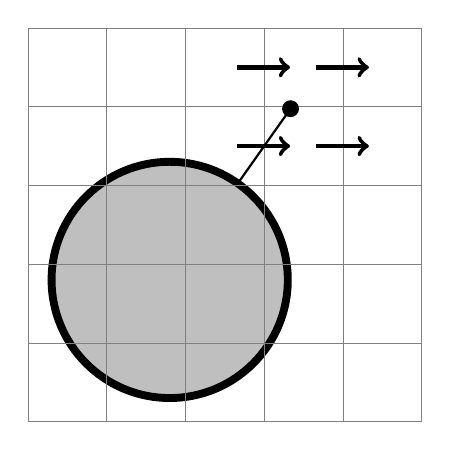
\begin{tikzpicture}
\draw[line width=1mm,fill=lightgray] (1.8,1.8) circle [radius=1.5];
\draw[help lines] (0,0) grid (5,5);
\draw[ultra thick,->] (2.66,4.5) -- (3.33,4.5);
\draw[ultra thick,->] (2.66,3.5) -- (3.33,3.5);
\draw[ultra thick,->] (3.66,4.5) -- (4.33,4.5);
\draw[ultra thick,->] (3.66,3.5) -- (4.33,3.5);
\draw[thick] (2.665,3.0255) -- (3.335,3.9745);
\draw[fill] (3.335,3.9745) circle [radius=0.1];
\end{tikzpicture}
\hspace{1cm}&\hspace{1cm}
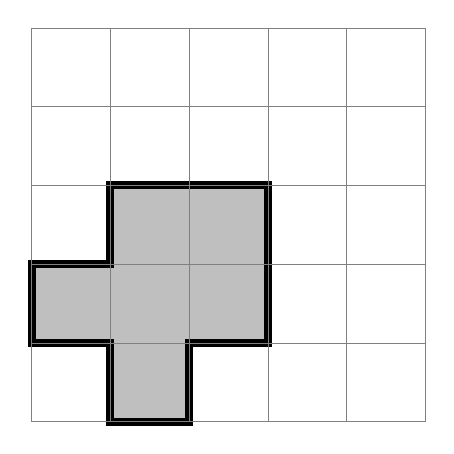
\begin{tikzpicture}
\draw[line width=1mm,fill=lightgray] (1,0) to (1,1) to (0,1) to (0,2) to (1,2) to (1,3) to (3,3) to (3,1) to (2,1) to (2,0) to (.95,0);
\draw[help lines] (0,0) grid (5,5);
\end{tikzpicture}
\end{tabular}
\caption{(Left) Desired geometry (circle). (Right) FDS representation---a cell is solid if more than half its volume is occupied by the desired geometry.}
\label{fig:circle}
\end{center}
\end{figure}


There are two shortcomings of the block geometry method.  First, it is zeroth-order accurate for curvilinear geometries \cite{Fadlun:temp}.
In other words, as the grid is refined---even after laborious reconstruction of the block geometry---we never recover the exact solution.  Second, creation of even simple geometries can be tedious. For example, users will go to incredible lengths to carve out rounded tunnels for circular ducts, a task that is fairly simple for most unstructured codes (not that the meshes tend to be much better!).

In direct forcing IBM, the force term in the momentum equation is set to drive a specific velocity component to a desired value.  In the block geometry approach (Fig.~\ref{fig:circle}, right), the impermeability condition is enforced by setting the normal component of velocity to zero on the solid surface. But as shown by Fadlun \cite{Fadlun:temp}, it is relatively simple to obtain a second-order solution for the velocity field: the velocity component is found from a linear interpolation between the velocity of the solid surface (no slip, impermeability) and a value at some distance normal to the surface.  This is illustrated on the left in Fig.~\ref{fig:circle}.  Away from the surface the staggered $u$ velocity components are interpolated to the point marked by the solid dot, which is twice the normal distance from the surface as the nearest velocity component.

More elaborate schemes exist to obtain the velocity near the surface \cite{Balaras:temp,Choi:temp,McDermott:temp}.  But the emphasis here is on the implementation of a scheme to transport heat and mass near thin obstructions (an issue yet to be addressed in the literature).  Therefore, Fadlun's simple interpolation method is sufficient for momentum.   In 2D, complex surfaces are constructed from a series of connected line segments. In 3D, surfaces are constructed from triangular facets.  Our goal is to minimize numerical diffusion across thin obstructions arbitrarily oriented relative to the Cartesian mesh.  The cause of this diffusion is discussed in more detail below.

In the following sections, we first discuss the linked-list data structure used to connect the surface elements to the grid, similar to the wall cell type used in the basic FDS scheme.  Next, we illustrate the momentum scheme for both simple and complex flow geometries.  We then discuss the unique issues faced by the FDS flow solver for simulating variable density flows with thin obstructions not aligned with the mesh.  Hopefully, we can develop a scheme that handles these problems!

\subsection{Data Structure}

\subsubsection{Block Geometry}

In the basic FDS method, a wall cell (WC) is one face of a gas phase cell.  A WC derived type stores the indices of the gas phase cell\footnote{Here I am not getting into the difference between wall cell and 1D in-depth derived types.  When I say WC, in most cases I mean precisely {\ct WC\%ONE\_D}.}.  It also stores face values of density, species mass fraction, and temperature, and the wall-normal cell dimension used to construct gradients.  The relevant variables in the code are:

\begin{table}[h!]
\begin{tabular}{ll}
{\ct WC\%IIG, WC\%JJG, WC\%KKG} & gas phase cell indices \\
{\ct WC\%UW}                    & wall-normal velocity component \\
{\ct WC\%RHO\_F}                & gas phase mass density at the wall \\
{\ct WC\%ZZ\_F}                 & lumped species mass fraction at the wall \\
{\ct WC\%TMP\_F}                & temperature at the wall \\
{\ct WC\%DN}                    & wall-normal cell dimension \\
{\ct WC\%IOR}                   & orientation from wall to cell center
\end{tabular}
\end{table}

The face values serve as Dirichlet boundary conditions.  If Neumann boundary conditions are needed, they are constructed from a one-sided difference.  For example, the temperature gradient at the wall is obtained from
\begin{equation}
\frac{\partial T}{\partial n} \approx \frac{T_g - T_f}{\delta n/2}
\end{equation}

\subsubsection{Complex Geometry}






\section{Verification Tests}

This section describes some of the test cases used to verify that FDS and Smokeview are computing
and visualizing unstructured geometric objects correctly.  This section will be used as source material for adding
more details to the various guides on how to setup unstructured geometries for use with FDS. (i.e. this section
is not intended to be included verbatim in the FDS User Guide).

\newcommand{\figheightD}{2.75in}

\subsection{geom\_simple.fds}
Figure \ref{fig:geom_simple} was created using the following \&GEOM namelist.
The {\ct VERTS}\ keyword is used to specify 3 vertices and the {\ct FACES}\ keyword
is used to specify the indices of the triangular face.

{\small
\begin{verbatim}
&GEOM ID='geom1',
VERTS=0.0,0.0,0.0,1.0,0.5,0.0,1.0,1.0,1.0,
FACES=1,2,3,
SURF_ID='surf1'/
\end{verbatim}
}

\begin{figure}
\begin{center}
\begin{tabular}{c}
 \includegraphics[width=4.0in]{SCRIPT_FIGURES/geom_simple}
  \end{tabular}
\end{center}
 \caption{A triangle created using 3 vertices and 1 face. Case: geom\_simple}
\label{fig:geom_simple}
\end{figure}

\subsection{geom\_azim.fds}
Figure \ref{fig:geom_azim} was created using the following \&GEOM namelists.
The {\ct AZIM}\ keyword is used to rotate the object about a vertical axis
centered at $(0,0,0)$.

{\small
\begin{verbatim}
&GEOM ID='geom1',
VERTS=0.0,0.0,0.0, 0.0,1.0,0.0, 0.0,1.0,1.0,
FACES=1,2,3,AZIM=0.0,SURF_ID='surf1'/

&GEOM ID='geom2',
VERTS=0.0,0.0,0.0, 0.0,1.0,0.0, 0.0,1.0,1.0,
FACES=1,2,3,AZIM=45.0,SURF_ID='surf2'/

&GEOM ID='geom3',
VERTS=0.0,0.0,0.0, 0.0,1.0,0.0, 0.0,1.0,1.0,
FACES=1,2,3,AZIM=90.0,SURF_ID='surf3'/
\end{verbatim}
}

\begin{figure}
\begin{center}
\begin{tabular}{c}
 \includegraphics[width=3.0in]{SCRIPT_FIGURES/geom_azim}
  \end{tabular}
\end{center}
 \caption{Three triangles generated at different azimuthal angles using the {\ct AZIM}\ keyword. Case: geom\_azim.fds}
\label{fig:geom_azim}
\end{figure}

\subsection{geom\_elev.fds}
Figure \ref{fig:geom_elev} was created using the following \&GEOM namelists.
The {\ct ELEV}\ keyword is used to rotate the object with respect to a horizontal plane
passing through $(0,0,0)$.

{\small
\begin{verbatim}
&GEOM ID='geom1',
VERTS=0.0,0.0,1.0,1.0,0.0,1.0,1.0,1.0,1.0,
FACES=1,2,3,ELEV=0,XYZ0=0.0,0.0,1.0,SURF_ID='surf1'/

&GEOM ID='geom2',
VERTS=0.0,0.0,1.0,1.0,0.0,1.0,1.0,1.0,1.0,
FACES=1,2,3,ELEV=45,XYZ0=0.0,0.0,1.0,SURF_ID='surf2'/

&GEOM ID='geom3',
VERTS=0.0,0.0,1.0,1.0,0.0,1.0,1.0,1.0,1.0,
FACES=1,2,3,ELEV=90,XYZ0=0.0,0.0,1.0,SURF_ID='surf3'/
\end{verbatim}
}

\begin{figure}
\begin{center}
\begin{tabular}{c}
 \includegraphics[width=3.0in]{SCRIPT_FIGURES/geom_elev}
  \end{tabular}
\end{center}
 \caption{Three triangles generated at different elevation angles using the {\ct ELEV}\ keyword. Case: geom\_elev.fds}
\label{fig:geom_elev}
\end{figure}

\subsection{geom\_scale.fds}
Figure \ref{fig:geom_scale} was created using the following \&GEOM namelists.
The {\ct SCALE}\ keyword is used to change the size of the object.

{\small
\begin{verbatim}
&GEOM ID='geom4',
VERTS=-2.0,0.0,0.0,-1.0,0.0,0.0,-1.0,0.0,1.0,
FACES=1,2,3,XYZ0=-2.0,0.0,0.0,SCALE=1.0,1.0,1.0,SURF_ID='surf1'/

&GEOM ID='geom4',
VERTS= 0.0,0.0,0.0,1.0,0.0,0.0,1.0,0.0,1.0,
FACES=1,2,3,XYZ0= 0.0,0.0,0.0,SCALE=1.0,1.0,2.0,SURF_ID='surf2'/

&GEOM ID='geom4',
VERTS= 2.0,0.0,0.0,3.0,0.0,0.0,3.0,0.0,1.0,
FACES=1,2,3,XYZ0= 2.0,0.0,0.0,SCALE=2.0,1.0,1.0,SURF_ID='surf3'/
\end{verbatim}
}

\begin{figure}
\begin{center}
\begin{tabular}{c}
 \includegraphics[width=6.0in]{SCRIPT_FIGURES/geom_scale}
  \end{tabular}
\end{center}
\caption{Three triangles generated at different scale sizes using the {\ct SCALE}\ keyword. Case: geom\_scale.fds}
\label{fig:geom_scale}
\end{figure}

\subsection{geom\_obst.fds}
Figure \ref{fig:geom_obst} was created using the following \&GEOM namelist.
The {\ct XB}\ keyword is used the same way to specify a block as on
a {\ct \&OBST}\ or {\ct \&VENT}\ line.

{\scriptsize
\begin{verbatim}
&GEOM ID='obst',SURF_ID='surf1', XB=-0.6,0.6,-0.6,0.6,-0.2,0.2,AZIM=90.0,ELEV=30.0 /
\end{verbatim}
}

\begin{figure}
\begin{center}
\begin{tabular}{c}
 \includegraphics[height=\figheightD]{SCRIPT_FIGURES/geom_obst}
  \end{tabular}
\end{center}
 \caption{A block generated using the {\ct XB}\ keyword.  The block is refined automatically to be consistent with the underlying grid resolution. Case: geom\_obst.fds}
\label{fig:geom_obst}
\end{figure}

\subsection{geom\_sphere1a.fds,...,geom\_sphere3f.fds}
Figure \ref{fig:geom_sphere} was created using {\ct LEVEL=n}\
in the following \&GEOM namelist
where {\ct n}\ ranges from 0 to 5.

{\scriptsize
\begin{verbatim}
&GEOM ID='sphere',SURF_ID='surf1',SPHERE_RADIUS=0.5,N_LEVELS=n,SPHERE_ORIGIN=0.0,0.0,0.0 /
\end{verbatim}
}

The {\ct N\_LEVELS}\ keyword is used
to specify the resolution of the sphere, larger {\ct N\_LEVELS}\ values result
in a more highly resolved sphere.{\ct LEVEL=0} produces a 20 sided sphere approximation, an icosahedron .
{\ct LEVEL=n} produces a sphere approximation with four times as many triangles as the
sphere produced with {\ct LEVEL=n-1}.
The {\ct SPHERE\_RADIUS}\ and {\ct SPHERE\_ORIGIN}\ keywords are used to specify
the size and location of the sphere.  This discretization technique results in equilateral triangles at each recursion level {(\em check to make sure this statement is true - when verified remove this comment)}.

\begin{figure}
\begin{center}
\begin{tabular}{cc}
 \includegraphics[width=3.5in]{SCRIPT_FIGURES/geom_sphere1a}&
 \includegraphics[width=3.5in]{SCRIPT_FIGURES/geom_sphere1b}\\
 LEVEL=0&LEVEL=1\\
 \includegraphics[width=3.5in]{SCRIPT_FIGURES/geom_sphere1c}&
 \includegraphics[width=3.5in]{SCRIPT_FIGURES/geom_sphere1d}\\
 LEVEL=2&LEVEL=3\\
 \includegraphics[width=3.5in]{SCRIPT_FIGURES/geom_sphere1e}&
 \includegraphics[width=3.5in]{SCRIPT_FIGURES/geom_sphere1f}\\
 LEVEL=4&LEVEL=5\\
  \end{tabular}
\end{center}
 \caption{Recursive sphere discretizations.  A sphere at a given level is
 obtained by splitting each triangle from the previous level into four parts and renormalizing added vertices. Cases: geom\_sphere1a.fds,...,geom\_sphere1f.fds}
\label{fig:geom_sphere}
\end{figure}

Figure \ref{fig:geom_sphere2a} was created by using {\ct N\_LAT}\ and {\ct N\_LONG}\ keywords in a {\ct \&GEOM}\ namelist
to split a sphere in latitudinal (north/south) and longitudinal (east/west) directions respectively. The minimum values of {\ct N\_LAT}\ and {\ct N\_LONG} permitted are 3 and 6.  This discretization technique results in triangles with high aspect ratios near the poles at higher discretization levels.

\begin{figure}
\begin{center}
\begin{tabular}{cc}
 \includegraphics[width=3.5in]{SCRIPT_FIGURES/geom_sphere3a}&
 \includegraphics[width=3.5in]{SCRIPT_FIGURES/geom_sphere3b}\\
 N\_LAT=3,N\_LONG=6&N\_LAT=6,N\_LONG=12\\
 \includegraphics[width=3.5in]{SCRIPT_FIGURES/geom_sphere3c}&
 \includegraphics[width=3.5in]{SCRIPT_FIGURES/geom_sphere3d}\\
 N\_LAT=12,N\_LONG=24&N\_LAT=24,N\_LONG=48\\
 \includegraphics[width=3.5in]{SCRIPT_FIGURES/geom_sphere3e}&
 \includegraphics[width=3.5in]{SCRIPT_FIGURES/geom_sphere3f}\\
 N\_LAT=48,N\_LONG=96&N\_LAT=96,N\_LONG=192\\
  \end{tabular}
\end{center}
 \caption{Latitude/Longitude sphere discretizations.  Spheres are
 split in longitudinal (east/west) and latitudinal (north/south) directions using the {\ct N\_LAT}\ and {\ct N\_LONG} keywords. Cases: geom\_sphere3a.fds,...,geom\_sphere3f.fds}
\label{fig:geom_sphere2a}
\end{figure}

%\geominput{geom_terrain.fds}
\subsection{geom\_terrain.fds}
Figure \ref{fig:geom_terrain} was created using the {\ct ZVALS}\ keyword.

\begin{figure}
\begin{center}
\begin{tabular}{c}
 \includegraphics[height=\figheightD]{SCRIPT_FIGURES/geom_terrain}
  \end{tabular}
\end{center}
 \caption{Elevations are defined on a rectangular array of grid points using the {\ct ZVALUES}\ keyword.  Case: gridgeom\_terrain.fds}
\label{fig:geom_terrain}
\end{figure}

\subsection{geom\_texture.fds}
Figure \ref{fig:geom_texture} was created using the following \&SURF and \&GEOM namelists.
The {\ct TEXTURE\_MAP}\ keyword on the {\ct \&SURF}\ is used to specify the name of the image
file used to texture map the geometric object.

{\small
\begin{verbatim}
&SURF ID='surf1',TEXTURE_MAP='nistleft.jpg',TEXTURE_WIDTH=0.6,TEXTURE_HEIGHT=0.2,COLOR='BLUE' /

&GEOM ID='texture',
VERTS=0.0,0.0,0.0, 1.0,0.0,0.0, 1.0,1.0,0.0,
FACES=1,2,3,SURF_ID='surf1'/
\end{verbatim}
}

\begin{figure}
\begin{center}
\begin{tabular}{c}
 \includegraphics[width=4.0in]{SCRIPT_FIGURES/geom_texture}
  \end{tabular}
\end{center}
 \caption{A texture is applied to a triangle. Case: geom\_texture.fds}
\label{fig:geom_texture}
\end{figure}

\subsection{geom\_texture2.fds}
Figure \ref{fig:geom_texture2} was created using the following \&SURF and \&GEOM namelists.
The {\ct TEXTURE\_MAP}\ keyword on the {\ct \&SURF}\ is used to specify the name of the image
file used to texture map the geometric object. This example has two textures.

{\small
\begin{verbatim}
&SURF ID='surf1' TEXTURE_MAP='nistleft.jpg',TEXTURE_WIDTH=0.6,TEXTURE_HEIGHT=0.2,COLOR='BLUE' /
&SURF ID='surf2',TEXTURE_MAP='grass.jpg',TEXTURE_WIDTH=0.6,TEXTURE_HEIGHT=0.2,COLOR='GREEN' /

&GEOM ID='texture',
VERTS=0.0,0.0,0.0, 1.0,0.0,0.0, 1.0,1.0,0.0,
FACES=1,2,3,SURF_ID='surf1'/

&GEOM ID='texture2',
VERTS=0.0,0.0,0.0, 1.0,1.0,0.0, 0.0,1.0,0.0,
FACES=1,2,3,SURF_ID='surf2'/
\end{verbatim}
}

\begin{figure}
\begin{center}
\begin{tabular}{c}
 \includegraphics[width=4.0in]{SCRIPT_FIGURES/geom_texture2}
  \end{tabular}
\end{center}
 \caption{Two texture maps are applied to two separate triangles.  Case: geom\_texture2.fds}
\label{fig:geom_texture2}
\end{figure}

\subsection{geom\_texture3a.fds, geom\_texture3b.fds, geom\_texture4a.fds, geom\_texture4b.fds}
The spheres in Figure \ref{fig:geom_texture3} were created using \&SURF and \&GEOM namelists similar to the following.

{\small
\begin{verbatim}
&SURF ID='surf1',TEXTURE_MAP='sphere_cover_03.png'COLOR='BLUE',
      TEXTURE_WIDTH=1.0,TEXTURE_HEIGHT=1.0/

&GEOM ID='sphere1',SURF_ID='surf1',
      N_LAT=50,N_LONG=50,SPHERE_RADIUS=0.25,SPHERE_ORIGIN=0.25,0.5,0.5,
      TEXTURE_ORIGIN=0.25,0.5,0.5,TEXTURE_MAPPING='SPHERICAL' /

&GEOM ID='sphere2',SURF_ID='surf3',
      N_LEVELS=3,SPHERE_RADIUS=0.25,SPHERE_ORIGIN=0.75,0.5,0.5,
      TEXTURE_ORIGIN=0.75,0.5,0.5,TEXTURE_MAPPING='SPHERICAL' /
\end{verbatim}
}

The {\ct TEXTURE\_MAP}\ keyword is used to specify the name of the image
file applied to the geometric object. The {\ct SPHERICAL}\ setting indicates that that the texture map image
is applied to the object using spherical coordinates.



\begin{figure}
\begin{center}
\begin{tabular}{cc}
 \includegraphics[width=3.5in]{SCRIPT_FIGURES/geom_texture3a}&
 \includegraphics[width=3.5in]{SCRIPT_FIGURES/geom_texture3b}\\
 \includegraphics[width=3.5in]{SCRIPT_FIGURES/geom_texture4a}&
 \includegraphics[width=3.5in]{SCRIPT_FIGURES/geom_texture4b}\\
 lat/long discretization&recursive discretization
  \end{tabular}
\end{center}
 \caption{Texture maps applied to spheres discretized using two different methods.
 The two sphere on the left are discretized by splitting the sphere along longitudinal (east/west) and latitudinal (north/south) directions.
 The two spheres on the right are discretized recursively starting with an icosahedron ( 20 sided polyhedron).  Texture maps applied to the top two sphere have 8 segments. Texture map applied to the bottom two spheres have 5 segments.  Cases: geom\_texture3a.fds, geom\_texture3b.fds, geom\_texture4a.fds, geom\_texture4b.fds}
\label{fig:geom_texture3}
\end{figure}

\subsection{geom\_arch.fds}
Figure \ref{fig:geom_arch} was created using VERTS and FACES keywords.

\begin{figure}
\begin{center}
\begin{tabular}{c}
 \includegraphics[width=4.0in]{SCRIPT_FIGURES/geom_arch}
  \end{tabular}
\end{center}
 \caption{An arch structure created with FACES and VERTS keywords.
 Case: geom\_arch.fds . }
\label{fig:geom_arch}
\end{figure}

%\subsection{geom\_time.fds}
%Figure \ref{fig:geom_time} was created using the following \&GEOM namelist.
%The {\ct AZIM}\ keyword is used to specify the initial rotational angle
%and the {\ct AXIM\_DOT}\ is used to specify that rate at which
%the azimuthal angle changes, in this  case 0.36 deg/s.
%
%{\small
%\begin{verbatim}
%&GEOM ID='geom4',
%      VERTS=0.0,0.0,0.0,0.0,1.0,0.0,0.0,1.0,1.0,
%      FACES=1,2,3,AZIM=0.0,AZIM_DOT=0.36,SURF_ID='surf1'/
%\end{verbatim}
%}
%
%\begin{figure}
%\begin{center}
%\begin{tabular}{ccc}
% \includegraphics[width=2.0in]{SCRIPT_FIGURES/geom_time_050}&
% \includegraphics[width=2.0in]{SCRIPT_FIGURES/geom_time_100}&
% \includegraphics[width=2.0in]{SCRIPT_FIGURES/geom_time_150}\\
% \SI{50.0}{s}&\SI{100.0}{s}&\SI{150.0}{s}
%  \end{tabular}
%\end{center}
% \caption{A triangle rotating about the scene center. Case: geom\_time.fds}
%\label{fig:geom_time}
%\end{figure}
%
%\subsection{geom\_time2.fds, geom\_time3.fds, geom\_time4.fds}
%Figure \ref{fig:geom_time2} was created using the following \&GEOM namelists.
%The {\ct AZIM}\ keyword is used to specify the initial rotational angle
%and the {\ct AXIM\_DOT}\ is used to specify that rate at which
%the azimuthal angle changes, in this  case 0.72 deg/s.
%The {\ct blade}\ object is used as components to create four blade objects
%{\ct blade1}, {\ct blade2}, {\ct blade3} and {\ct blade4} of the
%{\ct prop}\  object. The blades are positioned within the {\ct prop} using the {\ct DAZIM}\ keyword. Figures \ref{fig:geom_time3} and \ref{fig:geom_time4} were created similarly using rotation keywords to incline the geometric objects.
%
%{\small
%\begin{verbatim}
%&GEOM ID='blade',AZIM=0.0,AZIM_DOT=0.72
%VERTS=0.0,0.0,0.0,1.0,0.0,0.0,1.0,0.0,1.0,
%FACES=1,2,3,COMPONENT_ONLY=.TRUE.,SURF_ID='surf4'/
%
%&GEOM ID='blade1',GEOM_IDS(1)='blade',SURF_ID='surf1',COMPONENT_ONLY=.TRUE. /
%&GEOM ID='blade2',GEOM_IDS(1)='blade',SURF_ID='surf2',COMPONENT_ONLY=.TRUE. /
%&GEOM ID='blade3',GEOM_IDS(1)='blade',SURF_ID='surf3',COMPONENT_ONLY=.TRUE. /
%&GEOM ID='prop' GEOM_IDS(1)='blade1',DAZIM(1)=0.0,
%GEOM_IDS(2)='blade2',DAZIM(2)=90.0,
%GEOM_IDS(3)='blade1',DAZIM(3)=180.0,
%GEOM_IDS(4)='blade3',DAZIM(4)=270.0,
%\end{verbatim}
%}
%
%\begin{figure}
%\begin{center}
%\begin{tabular}{ccc}
% \includegraphics[width=2.0in]{SCRIPT_FIGURES/geom_time2_050}&
% \includegraphics[width=2.0in]{SCRIPT_FIGURES/geom_time2_100}&
% \includegraphics[width=2.0in]{SCRIPT_FIGURES/geom_time2_150}\\
% \SI{50.0}{s}&\SI{100.0}{s}&\SI{150.0}{s}
%  \end{tabular}
%\end{center}
% \caption{Four triangles defined as a group rotating about the scene center. A Case: geom\_time2.fds}
%\label{fig:geom_time2}
%\end{figure}
%
%\begin{figure}
%\begin{center}
%\begin{tabular}{ccc}
% \includegraphics[width=2.0in]{SCRIPT_FIGURES/geom_time3_050}&
% \includegraphics[width=2.0in]{SCRIPT_FIGURES/geom_time3_100}&
% \includegraphics[width=2.0in]{SCRIPT_FIGURES/geom_time3_150}\\
% \SI{50.0}{s}&\SI{100.0}{s}&\SI{150.0}{s}
%  \end{tabular}
%\end{center}
% \caption{Four inclined triangles defined as a group rotating and about the scene center. A Case: geom\_time3.fds}
%\label{fig:geom_time3}
%\end{figure}
%
%\begin{figure}
%\begin{center}
%\begin{tabular}{ccc}
% \includegraphics[width=2.0in]{SCRIPT_FIGURES/geom_time4_050}&
% \includegraphics[width=2.0in]{SCRIPT_FIGURES/geom_time4_100}&
% \includegraphics[width=2.0in]{SCRIPT_FIGURES/geom_time4_150}\\
% \SI{50.0}{s}&\SI{100.0}{s}&\SI{150.0}{s}
%  \end{tabular}
%\end{center}
% \caption{Two sets of four triangles rotating about the scene center. Each set of 4 triangles are defined as a group. Case: geom\_time4.fds}
%\label{fig:geom_time4}
%\end{figure}

%\subsection{geom\_slice.fds}
%The slice file in Figure \ref{fig:geom_slice} was generated using the {\tt SLICETYPE}\ keyword on a {\tt \&SLCF}\ namelist statement as in
%{\footnotesize
%\begin{verbatim}
%&SLCF PBY=0.75,QUANTITY='TEMPERATURE',CELL_CENTERED=.TRUE., SLICETYPE='EXCLUDEGEOM' /.
%\end{verbatim}
%}
%
%\noindent The {\tt SLICETYPE}\ keyword is used to specify the type of slice generated.  For example, a slice consisting of only cutcells, a slice  including the effects of immersed geometry, a slice ignoring immersed geometry and a slice output using the original slice file format.  These choices are documented in Table \ref{table:slicetype}.
%
%\begin{table}
%\caption{Description of {\tt SLICETYPE}\ values used on a {\tt \&SLCF}\ namelist statement }
%\begin{tabular}{|l|l|}
%  \hline
%Keyword& Description\\
%\hline
%STRUCTURED&generate slice using original  file format\\
%CUTCELL&output only triangle faces associated with  cutcells\\
%INCLUDEGEOM&include immersed geometry when generating a slice file\\
%EXCLUDEGEOM&ignore immersed geometry when generating a slice file\\
%\hline
%\end{tabular}
%\label{table:slicetype}
%\end{table}
%
%\begin{figure}
%\begin{center}
%\begin{tabular}{cc}
% \includegraphics[width=3.0in]{SCRIPT_FIGURES/geom_slice_slice_000}&
% \includegraphics[width=3.0in]{SCRIPT_FIGURES/geom_slice_slice_020}\\
% \SI{0.0}{s}&\SI{20.0}{s}
%  \end{tabular}
%\end{center}
% \caption{Slice file generated using the geometry file format Case: geom\_slice.fds.  The two triangles are an immersed object with boundary file temperature data displayed on its surface.}
%\label{fig:geom_slice}
%\end{figure}

%\subsection{geom\_sphere2.fds}
%Figure \ref{fig:geom_sphere2b} tests motion of a scaled,  moving, rotating sphere. The sphere was scaled using {\ct SCALE=0.6,0.4,0.2}\, placed initially at the right side of the domain using {\ct XYZ=10.0,0.5,1.0}, translated to the left and down using {\ct XYZ\_DOT=-0.01,0.0,-0.001} and rotated using {\ct GROTATE\_DOT=0.36}.  The axis of rotation was specified using {\ct GAXIS=0.0,1.0,0.0}.
%
%\begin{figure}
%\begin{center}
%\begin{tabular}{c}
%\includegraphics[width=6.0in]{SCRIPT_FIGURES/geom_sphere2_000}\\
%\includegraphics[width=6.0in]{SCRIPT_FIGURES/geom_sphere2_200}\\
%\includegraphics[width=6.0in]{SCRIPT_FIGURES/geom_sphere2_400}\\
%\includegraphics[width=6.0in]{SCRIPT_FIGURES/geom_sphere2_600}\\
%\includegraphics[width=6.0in]{SCRIPT_FIGURES/geom_sphere2_800}\\
%\includegraphics[width=6.0in]{SCRIPT_FIGURES/geom_sphere2_1000}
%  \end{tabular}
%\end{center}
% \caption{Motion of a scaled, moving, rotating sphere.  Case: geom\_sphere2.fds}
%\label{fig:geom_sphere2b}
%\end{figure}

%\subsection{geom\_sphere\_fire.fds}
%Figure \ref{fig:geom_sphere_fire} tests visualization of a boundary file data on a sphere.

%\begin{figure}
%\begin{center}
%\begin{tabular}{cc}
%\includegraphics[width=3.0in]{SCRIPT_FIGURES/geom_sphere_fire_000}&
%\includegraphics[width=3.0in]{SCRIPT_FIGURES/geom_sphere_fire_020}\\
%\SI{0.0}{s}&\SI{2.0}{s}\\
%\includegraphics[width=3.0in]{SCRIPT_FIGURES/geom_sphere_fire_040}&
%\includegraphics[width=3.0in]{SCRIPT_FIGURES/geom_sphere_fire_060}\\
%\SI{4.0}{s}&\SI{6.0}{s}\\
%\includegraphics[width=3.0in]{SCRIPT_FIGURES/geom_sphere_fire_080}&
%\includegraphics[width=3.0in]{SCRIPT_FIGURES/geom_sphere_fire_100}\\
%\SI{8.0}{s}&\SI{10.0}{s}\\
% \end{tabular}
%\end{center}
%\caption{Boundary file data visualized on a sphere.  Case: geom\_sphere\_fire.fds}
%\label{fig:geom_sphere_fire}
%\end{figure}

%Figure \ref{fig:geom_sphere2_fire} tests visualization of a boundary file data on a moving sphere.

%\begin{figure}
%\begin{center}
%\begin{tabular}{cc}
% \includegraphics[width=3.0in]{SCRIPT_FIGURES/geom_sphere2_fire_000}&
% \includegraphics[width=3.0in]{SCRIPT_FIGURES/geom_sphere2_fire_020}\\
% \SI{0.0}{s}&\SI{2.0}{s}\\
% \includegraphics[width=3.0in]{SCRIPT_FIGURES/geom_sphere2_fire_040}&
% \includegraphics[width=3.0in]{SCRIPT_FIGURES/geom_sphere2_fire_060}\\
% \SI{4.0}{s}&\SI{6.0}{s}\\
% \includegraphics[width=3.0in]{SCRIPT_FIGURES/geom_sphere2_fire_080}&
% \includegraphics[width=3.0in]{SCRIPT_FIGURES/geom_sphere2_fire_100}\\
% \SI{8.0}{s}&\SI{10.0}{s}\\
%  \end{tabular}
%\end{center}
% \caption{Boundary file data visualized on a moving sphere.  Case: geom\_sphere2\_fire.fds}
%\label{fig:geom_sphere2_fire}
%\end{figure}


\subsection{Cut-cell definition around immersed cone: split cells, piercing and alignment}


\subsection{Cut-cell definition around sphere: serial performance and parallel scaling}


\subsection{Explicit-implicit time integration for scalar transport}


\subsubsection{Temporal Error analysis for variable density projection}

\label{sec:saad_cc_temporal_error}

This case is a variation of problem \ref{sec:saad_temporal_error} for a domain that includes an imposed cut-cell region, where the cut-cells have same geometry as regular cells. The problem allows us to verify the temporal accuracy of our scalar transport implementation for cut-cells. The problem is defined by the advection of a non-reacting mixture of two fluids with different densities (10:1 ratio) in one cartesian direction. Zero diffusivity is prescribed. For the problem definition and temporal error computation details, we refer the reader to problem \ref{sec:saad_temporal_error}.
The domain is defined by a mesh containing $N_x=512$ cells in the $x$ direction, where the domain $x=[-1,1]$. Also, four cells are defined in the $y$ direction as required by the FFT Poisson solver. Note that the problem defined is one-dimensional in $x$. 
On this domain, cut-cells with same shape and size of regular cells are defined in the space $x=[-0.5,0.5]$. The test verifies that the implementation details of this cut-cell region does not affect the temporal order of accuracy seen on the default verification case of section \ref{sec:saad_temporal_error}.

\title{Temporal order of accuracy}

Six cases are defined for this test:
%
\begin{enumerate}
 \item[a]  Three correspond to default FDS DNS flux limiter and default explicit Strong Stability Preserving Runge Kutta (SSPRK2) time integration in cells not covered by cut-cells, plus Godunov flux limiter and explicit SSPRK2 time integration in cut-cell region, for CFL numbers $0.25$, $0.125$, $0.0625$. These cases are defined in {\ct /Complex\_Geometry/saad\_CC\_explicit\_*.fds}. 
 
  \item[b] The other three cases correspond to default flux limiter and time integration in cells not covered by cut-cells, plus Godunov flux limiter and implicit time integration in cut-cell region for the same CFL numbers. The implicit integration on the cut-cell region is done applying an Backward Euler step in the predictor, and Trapezoidal Rule on the corrector step. The imposition of boundary conditions for the implicit region in domain and explicit-implicit (EXIM) boundaries follows the technical notes in section \ref{sec:exim_scalar_transport} of the Technical Reference Guide. These cases are defined in {\ct /Complex\_Geometry/saad\_CC\_implicit\_*.fds}.
  
\end{enumerate}
%

Same procedure as explained in section  \ref{sec:saad_temporal_error} is used to define the temporal order of accuracy $p$. As noted there, this procedure filters out the spatial error from the computed temporal convergence. Initial and final fields for temperature and mixture fraction for the smallest integration time step are shown in the top figures of Fig.~\ref{fig:saad_cc_temporal_order}. Fields advect to the right with unitary velocity. The two bottom figures show the order $p$ computed point wise in the $x$ direction for explicit and implicit time integration on the cut-cell region. Deviations from $p \simeq 2$ are dependent on the formula used to compute $p$, as explained in section~\ref{sec:saad_temporal_error}. 
The $l_2$ norm of $p$ computed pointwise for explicit integration in cut-cells is \input{../FDS_Verification_Guide/SCRIPT_FIGURES/saad_CC_explicit_l2_norm}\!, and for implicit time integration of scalars on these is  \input{../FDS_Verification_Guide/SCRIPT_FIGURES/saad_CC_implicit_l2_norm}\!. 

\begin{figure}[ht]
\centering
\includegraphics[width=.49\textwidth]{../FDS_Verification_Guide/SCRIPT_FIGURES/saad_CC_explicit_Z.pdf}
\includegraphics[width=.49\textwidth]{../FDS_Verification_Guide/SCRIPT_FIGURES/saad_CC_explicit_rho.pdf}
\includegraphics[width=.49\textwidth]{../FDS_Verification_Guide/SCRIPT_FIGURES/saad_CC_explicit_temporal_order_rho.pdf}
\includegraphics[width=.49\textwidth]{../FDS_Verification_Guide/SCRIPT_FIGURES/saad_CC_implicit_temporal_order_rho.pdf}
\caption[The {\ct saad CC} temporal order test case]{Temporal order for a variable-density projection on domain including cut-cell region.  (Upper-left) Initial and final field for mixture fraction, explicit time integration on cut-cells.  (Upper-right) Initial and final field for density, explicit time integration on cut-cells.  (Lower-left) $p$ computed pointwise for density at final time, explicit integration on cut-cells. (Lower-right) $p$ computed pointwise for density at final time, implicit time integration on cut-cells.  Fluctuations are due to degenerate points in the formula for $p$.}\label{fig:saad_cc_temporal_order}
\end{figure}


\subsubsection{Variable-Density manufactured solution}






\subsection{Immersed boundary method on manufactured solution around rotated cube}





\subsection{Conservation test of isothermal helium plume around sphere}





\subsection{Parallel consistency test of helium plume around sphere, 1 mesh vs. 3 meshes}




\subsection{Consistency test for OBST and GEOM of flow around heated cubes}




%\subsection{Flow around heated curved pipe or something like that}




\section{Validation Tests}

\subsection{Vettori fire on sloped ceiling compartment experiments}





\subsection{Lattimer flow around inclined wall experiments}





\subsection{Askervein Hill}







%As we move toward complex shapes immersed within the Cartesian mesh, to the extent possible we have tried to maintain a correspondence with the WC data type.  The analog in the new approach is, in 3D, a triangular facet, FC. This choice was made for the following reasons:
%\begin{enumerate}[{\,\,\,\,(}a{)}]
%\item For simplicity, we wanted to restrict ourselves to one generic element type.
%\item Curvilinear surfaces can be approximated to second-order accuracy with linear elements.
%\item Three points are unambiguously planar.
%\item Algorithms for triangle/box intersection are readily available.
%\end{enumerate}
%
%Note that a basic WC face must be constructed from two FC faces (see Fig.~\ref{fig:facetcell}), thus doubling computational effort for the same resolution.  The FC approach makes up for this deficiency with the following benefits:
%\begin{enumerate}[{(}i{)}]
%\item We have the flexibility to create arbitrarily complex shapes.
%\item The resolution of the solid surface need not be the same as the gas phase.  When coarser resolution is permissible, we achieve a cost savings.
%\end{enumerate}
%
%%The first item may be obvious, but the second deserves elaboration. For many objects in the scenario, the boundary conditions may not change much or may not be important enough to finely resolve.  Suppose there is a door that is only partially open (say 45$^\circ$ angle) and the gas phase resolution within the room is 10 cm.  A standard doorway in the U.S. is 91 cm by 203 cm.  Therefore, resolving each gas phase cell with a wall cell on the door would require roughly $9 \times 20 \times 2 = 360$ facets.  But if detailed resolution of the door is unnecessary, we can get away with only 2 facets (see Fig.~\ref{fig:opendoor}).
%
%\begin{figure}
%\begin{center}
%\begin{tikzpicture}
%
%\draw (0,0)--(0,3);
%\draw (0,3)--(3,3);
%\draw (3,3)--(3,0);
%\draw (3,0)--(0,0);
%
%\draw (1,4)--(4,4);
%\draw (4,4)--(4,1);
%
%\draw (0,3)--(1,4);
%\draw (3,3)--(4,4);
%\draw (3,0)--(4,1);
%
%\draw (0,0)--(3,3);
%\draw (3,3)--(4,1);
%\draw (1,4)--(3,3);
%
%\end{tikzpicture}
%
%\caption{Triangular facets covering a cubic cell.  Two facets are needed for each face, as opposed to one wall cell.}
%\label{fig:facetcell}
%\end{center}
%\end{figure}
%
%
%%\begin{figure}
%%\begin{center}
%%\begin{tikzpicture}[scale=0.75]
%%
%%\draw (0,6) -- (2,8);
%%\draw (0,0) -- (2,2);
%%
%%\draw (12,6) -- (10,8);
%%\draw (12,0) -- (10,2);
%%
%%\draw (2,8) -- (10,8);
%%\draw (2,8) -- (2,2);
%%\draw (10,8) -- (10,2);
%%
%%\draw (4,6.5) -- (6.5,6.5);
%%\draw (4,2) -- (4,6.5);
%%\draw (2,2) -- (4,2);
%%\draw (6.5,2) -- (10,2);
%%
%%\draw (0,0) -- (0,6);
%%\draw (12,0) -- (12,6);
%%\draw (0,0) -- (12,0);
%%
%%\draw[help lines] (1.499,1.499) grid [step=.25cm] (10.5,7.5);
%%
%%\draw[help lines,fill=white] (5,1) to (5,5.5) to (6.5,2) to (5,1);
%%\draw[help lines,fill=white] (6.5,6.5) to (5,5.5) to (6.5,2) to (6.5,6.5);
%%
%%\draw (6.5,2) -- (6.5,6.5);
%%\draw (6.5,6.5) -- (5,5.5);
%%\draw (6.5,2) -- (5,1);
%%\draw (5,1) -- (5,5.5);
%%\draw (5,5.5) -- (6.5,2);
%%
%%\draw[help lines] (5.7499,1.5) grid [step=.25cm] (7.5,7.5);
%%
%%\end{tikzpicture}
%%
%%\caption{Partially open door composed of two facets, illustrating that the solid resolution may be coarser than the gas phase resolution.}
%%\label{fig:opendoor}
%%\end{center}
%%\end{figure}
%
%
%\subsection{Momentum}
%\label{sec:momentum}
%
%Consider the following semi-implicit (fractional step) update for the $i$th component of momentum:
%\begin{equation}
%\label{eqn:mom}
%\frac{u_i^{n+1} - u_i^n}{\delta t} = -\left(F_i^n + \frac{\delta H^{n+1}}{\delta x_i}\right)
%\end{equation}
%This is a fractional step method because a Poisson equation is solved to obtain the pressure term, $H$ (not discussed here). In a direct-forcing immersed boundary method, the force term is replaced by
%\begin{equation}
%\label{eqn:force}
%F_i^* = - \left( \frac{u_i^{ibm} - u_i^n}{\delta t} + \frac{\delta H^*}{\delta x_i}\right)
%\end{equation}
%which drives the velocity component $u_i^{n+1}$ toward $u_i^{ibm}$.  The superscript asterisk indicates that the initial guess for the pressure term is taken from the previous time step.  The update may be iterated to drive the error between $u_i^{n+1}$ and $u_i^{ibm}$ to a desired tolerance.  Note, however, that when this approach is embedded in a second-order predictor-corrector scheme the error in most cases is remarkably small when $H^n$ is used in the force term (no iteration).
%
%\subsubsection{Block Geometry}
%
%For the basic block geometry method used in FDS, the impermeability condition at a surface is enforced by setting $u_i^{ibm} = 0$. If mass transfer is present the surface-normal IBM velocity component is set to $u_i^{ibm} = u_n$, where $u_n$ is the wall-normal component of velocity satisfying the scalar transport equation.  Note that $u_n$ is stored as {\ct WC\%UW} in the code.
%
%\subsubsection{Complex Geometry}
%
%For complex geometry the surface usually does not align itself with the face of a Cartesian grid cell. A given velocity component, therefore, is not on a boundary, but must still satisfy the governing equations subject to the prescribed boundary conditions (position and properties of the surface).  The essential task of a direct-forcing immersed boundary method is to set $u_i^{ibm}$ to achieve a stable and accurate numerical solution as well as an adequate representation of the local flow physics (surface stress, pressure gradient, etc.) without the luxury of infinitely high resolution.
%
%In FDS, there are three IBM options for momentum, set by, for example,
%\small
%\begin{verbatim}
%&MISC IMMERSED_BOUNDARY_METHOD=1/ ! options are 0,1,2
%\end{verbatim}
%\normalsize
%Following is a brief description of each option. The basic linear interpolation method of Fadlun \cite{Fadlun:temp} is given by option (1), and will be used for the examples to follow later in this paper. Refer to the diagram in Fig.~\ref{fig:position_definitions} for position definitions.
%
%\paragraph{\ct IMMERSED\_BOUNDARY\_METHOD=0}
%
%The velocity component force term is unaltered if it falls on the positive side of the surface.  Let $\mathbf{x}_{velo}$ denote the location of the velocity component, $\mathbf{v}_i, (i=1,2,3)$ are the vertices of a face, $\mathbf{n} = (\mathbf{v}_2-\mathbf{v}_1) \times (\mathbf{v}_3-\mathbf{v}_1)$ is the face normal, and let $\mathbf{r} \equiv \mathbf{x}_{velo} - \mathbf{v}_1$ (any of the vertices will do); then if $\delta n =\mathbf{r} \cdot \mathbf{n} > 0$ the velocity component is processed as usual; if the dot product is negative the velocity is ``inside'' the obstruction and is set to zero.  This effectively leads to a zeroth-order (Lego block) representation of the surface.
%
%\paragraph{\ct IMMERSED\_BOUNDARY\_METHOD=1}
%
%The basic linear interpolation scheme of Fadlun starts by identifying a point $\mathbf{x}_{int}$ (see Fig.~\ref{fig:position_definitions}) which is twice the normal distance from the surface as the position of the velocity component, $\mathbf{x}_{velo}$.  The value $u_i(\mathbf{x}_{int}) = u_{i,int}$ is found from a trilinear interpolation of the neighboring staggered velocity component values from the previous time step.  The value of $u_i^{ibm}$ is then taken from a linear interpolation between $u_{i,int}$ and the wall value of the velocity component, $u_{i,w}$ (usually zero).  Thus, $u_i^{ibm} = \frac{1}{2}(u_{i,int} + u_{i,w})$.
%
%\paragraph{\ct IMMERSED\_BOUNDARY\_METHOD=2}
%
%Here the linear profile is replaced by a prescribed wall-normal profile for the mean streamwise velocity.  This requires that we first define a new streamwise coordinate system.  Referring to Fig.~\ref{fig:position_definitions}, let $\mathbf{e}_i, (i=1,2,3)$ define an orthonormal set of basis vectors for our Cartesian grid system and let $\mathbf{\bar{e}}_i, (i=1,2,3)$ define the new streamwise system where $\mathbf{\bar{e}}_1$ is the streamwise direction and $\mathbf{\bar{e}}_3$ is the wall-normal direction.  It is useful to define the new system so that the velocity component in $\mathbf{\bar{e}}_2$ is always zero.  This is achieved as follows: Define a tangent vector $\mathbf{t} \equiv \mathbf{n} \times (\mathbf{u} - \mathbf{u}_w)$ where $\mathbf{u}_w$ is the velocity of the wall (usually zero) and $\mathbf{n}$ is a wall-normal vector. The streamwise basis vector is then found from $\mathbf{\hat{s}} = \mathbf{\hat{t}} \times \mathbf{\hat{n}}$.  The hat represents a unit normal, e.g., $\mathbf{\hat{n}} \equiv \mathbf{n}/|\mathbf{n}|$.  The new streamwise system is then given by $\mathbf{\bar{e}_1}=\mathbf{\hat{s}}$, $\mathbf{\bar{e}_2}=\mathbf{\hat{t}}$, and $\mathbf{\bar{e}_3}=\mathbf{\hat{n}}$. (To conform to the convention used in the atmospheric community, in FDS, the ``vertical'' or surface-normal component is taken as the ``$z$'' component.  Hence, 2D flows are in the $x-z$ plane.)  The elements of the directional cosine matrix are now simply $a_{ij} = \mathbf{e}_i \cdot \mathbf{\bar{e}}_j$.  Velocity vectors may be transformed from the grid system to the streamwise system via $\bar{u}_k = a_{ik} u_i$ and back again via $u_i = a_{ik} \bar{u}_k$ (see, e.g., \cite{Pope:2000} Appendix B).
%
%To evaluate the streamwise profile, all three staggered velocity components are interpolated to $\mathbf{x}_{int}$ and the vector is transformed into the streamwise system.  The streamwise component at $\mathbf{x}_{int}$ is used to define the profile $f(n)$, which is then used to specify the streamwise component at the position of interest ($\mathbf{x}_{velo}$ in the grid system).  Thus, we obtain $\bar{u}_1^{ibm} = f(\delta n)$.  Here note that the bar indicates we are in the streamwise coordinate system.  We need to specify the other two components before we can transform back to the grid system.  As mentioned, the tangential component is zero by construction. Specification of the normal component is currently an active area of research \cite{Choi:2007:temp}.  What complicates matters is that we have two invariants to satisfy: (1) the divergence and (2) the kinetic energy. The kinetic energy is the easier of the two because it does not involve differences.  Still, since all we know from the model is a mean profile, some sort of \emph{ad hoc} assumption must be made.  Given $k_{int}=\frac{1}{2}u_i u_i$ at $\mathbf{x}_{int}$, we use a linear interpolation to determine $k(\delta n) = \frac{1}{2}(k_{int} + k_w)$, where $k_w$ is the kinetic energy at the wall (usually zero).  The magnitude of the normal component is then found from $|\bar{u}_3^{ibm}| = +\sqrt{2k(\delta n) - (\bar{u}_1^{ibm})^2}$.  Finally, the component value of interest is obtained from the transformation $u_i^{ibm} = a_{ik} \bar{u}_k^{ibm}$, where only the $i$th component is retained at the staggered location.
%
%\begin{figure}
%\begin{center}
%\begin{tikzpicture}[scale=1.25]
%
%\draw [fill=lightgray] (0.2,0.5) -- (2.2,3.8) -- (4.5,3.1) -- (0.2,0.5);
%
%\draw[help lines] (-3,-1) grid [step=2cm] (5,7);
%
%\draw (0.30,0.25) node {$\mathbf{v}_1$};
%\draw (4.80,3.10) node {$\mathbf{v}_2$};
%\draw (2.20,4.00) node {$\mathbf{v}_3$};
%
%\draw [->, very thick, >=latex] (-2.5,5.0) -- (-1.5,5.0);
%\draw [->, very thick, >=latex] (-2.5,3.0) -- (-1.5,3.0);
%\draw [->, very thick, >=latex] (-0.5,5.0) -- (0.5,5.0);
%\draw [->, very thick, >=latex] (-0.5,3.0) -- (0.5,3.0);
%\draw (0.5,3.3) node {$\mathbf{x}_{velo}$};
%
%\draw [->, very thick, >=latex] (0.2,0.5) -- (0.0,3.0);
%\draw (-0.15,1.8) node {$\mathbf{r}$};
%
%\draw [->, very thick, >=latex] (0.2,0.5) -- (-1,2.0);
%\draw (-0.5,1.0) node {$\mathbf{n}$};
%
%\draw [->, >=*] (1.1,1.545) -- (-1.3,4.7);
%\draw (-1.5,4.3) node {$\mathbf{x}_{int}$};
%
%\draw [|-] (0.9,1.37) -- (0.57,1.8);
%\draw [-|] (0.24,2.25) -- (-0.19,2.85);
%\draw (.4,2.02) node {$\delta n$};
%
%\draw [->, very thick, >=latex] (1.08,1.55) -- (2.35,1.55);
%\draw [->, very thick, >=latex] (1.1,1.545) -- (0.45,2.4);
%\draw [->, very thick, >=latex] (1.1,1.545) -- (1.75,2.6);
%\draw (2.9,1.55) node {$\mathbf{\hat{s}} \, (\mathbf{\bar{e}}_1)$};
%\draw (1.9,2.60) node {$\mathbf{\hat{t}}$};
%\draw (0.6,2.60) node {$\mathbf{\hat{n}}$};
%
%\draw [->, very thick, >=latex] (-2,0) -- (-2,1);
%\draw [->, very thick, >=latex] (-2,0) -- (-1,0);
%\draw (-0.9,-0.25) node {$\mathbf{e}_1$};
%\draw (-2.35,1) node {$\mathbf{e}_3$};
%
%\draw (1,4.7) .. controls (2.5,2) .. (1.1,1.545);
%\draw [->] (-1.15,4.500) -- (1.10,4.500);
%\draw [->] (-0.58,3.750) -- (1.52,3.750);
%\draw [->] ( 0.20,3.003) -- (1.90,3.003);
%\draw [->] ( 0.54,2.280) -- (2.15,2.280);
%\draw [->] ( 0.90,1.800) -- (1.80,1.800);
%\draw (1.5,5.0) node {$f(n)$};
%
%\end{tikzpicture}
%
%\caption{Position definitions for a single facet.  The function $f(n)$ represents the mean streamwise velocity profile in the wall-normal direction.}
%\label{fig:position_definitions}
%\end{center}
%\end{figure}
%
%\paragraph{Remark} As can be seen, in going from IBM methods 0 to 2 the level of complexity increases significantly.  For the remainder of this paper, we utilize method 1.  The main reason is that our focus here is on the additional complexities that arise with considering heat and mass transfer near infinitely thin obstructions.
%
%%\subsubsection{Convergence of IBM 1}
%%\label{sec:momentum_convergence}
%%
%%In this section we show second-order convergence for IBM 1 by examining the 2D flow near a rotating disk.
%
%\subsection{Heat and Mass Transfer}
%
%This is where the formulation gets tricky.  Both heat and mass transfer present challenges for a typical IBM formulation.  For heat transfer, numerical diffusion from the gas phase domain into the solid domain implies that global energy is not conserved.  For mass transfer, when considering the ``mixed is burnt'' model for combustion chemistry, any numerical diffusion of reactant species across a solid boundary can be fatal to a calculation.  For these reasons, we have chosen to implement a hybrid cutcell immersed boundary method (CIBM), where the cutcells on the immersed boundary surface are treated by an unstructured finite volume solver for heat and mass transport.  This ensures strict conservation of mass and energy in the fluid domain.
%
%\subsubsection{To-Do List}
%
%\begin{enumerate}
%\item Identify cutcells.  Find the Cartesian cells that intersect with solid tet volumes.  To handle zero thickness obstructions we either need the ability to treat facets by themselves or we may allow ``volumes'' with zero volume.  To be discussed.
%\item Compute cutcell (CC) volumes.  Let $V_{cell}$ denote the volume of the Cartesian cell.  Let $V_{tet}$ denote a tetrahedral volume.  The cutcell volume is $V_{cc} = V_{cell} - ( V_{cell} \cap V_{tet} )$.
%\item Merge small cells.  If $V_{cc} < V_{tol}$, merge with a neighboring cell (Cartesian cell or cutcell).  This limits CFL time step restrictions.
%\item Compute surface areas and unit normal vectors for final cutcell volumes.
%\item Interpolate scalars (density, mass fractions, temperature) to CC volume faces (see below).
%\item Interpolate velocity components to CC faces (see below).
%\item Update finite volumes equations (see below).
%\item Construct Cartesian divergence from CC divergence integral (see below).
%\item Update Poisson equation as usual (see FDS Tech Guide).
%\item Reconstruct velocity field to satisfy projection and CC constraints (see below).
%\end{enumerate}
%
%\newpage
%
%\subsubsection{FDS Grid Data Structure}
%
%
%In the following, variables and proposed data lists for cut-cells and faces to be used in the FDS CCIBM code are described. Data structures from the prototype Matlab code and linked list definitions from the current FDS IBM implementation are included for clarity. Names can be changed if there are issues with the existing FDS namespace, etc. Also, we keep it general for now.
%
%
%\subsubsection*{Some type defining and indexing parameters:}
%
%The following parameters are used in defining the type (or status) of cell or cell face on Cartesian grid or solid surfaces: \\
%\texttt{INTEGER, PARAMETER :: GASPHASE     = -1} \\
%\texttt{INTEGER, PARAMETER :: CUTCF         =   0} \\
%\texttt{INTEGER, PARAMETER :: SOLID              =   1} \\
%\texttt{INTEGER, PARAMETER :: INBOUNDARY =   2} \\
%
%
%
%\subsubsection*{New Cartesian grid variables:}
%
%- \textit{Cell-centered} variables for cell-type identification, unknown numbering, etc.:  \\
% \texttt{INTEGER} \texttt{CCVAR(I,J,K,ICVAR)}: Here,  \texttt{ICVAR} can be equal to:   \\
%%
%\begin{itemize}
%
%  \item \texttt{INTEGER, PARAMETER :: IGSC = 1} such that: \\
%           - \texttt{CCVAR(I,J,K,IGSC) == GASPHASE} is a regular \texttt{GASPHASE} cell. \\
%           - \texttt{CCVAR(I,J,K,IGSC) == CUTCF} is a cut-cell, i.e. cell transversed by the solid wet surface. \\
%           - \texttt{CCVAR(I,J,K,IGSC) == SOLID} is a regular cell immersed completely in the solid region.
%
%  \item \texttt{ICVAR} can take other values (2, 3,... to be added later) to map unknowns to \texttt{CUT\_CELL} data, linear systems, etc.
%
%
%\end{itemize}
%%
%- \textit{Face-centered} variables for face-type identification, generating data necessary for matrix and vector building (face based),  etc.:  \\
%\texttt{INTEGER} \texttt{FCVAR(I,J,K,IFVAR)}: Here,  \texttt{IFVAR} can be equal to:   \\
%%
%\begin{itemize}
%
%  \item \texttt{INTEGER, PARAMETER :: FGSC = 1} such that: \\
%           - \texttt{FCVAR(I,J,K,FGSC) == GASPHASE} is a regular \texttt{GASPHASE} face. \\
%           - \texttt{FCVAR(I,J,K,FGSC) == CUTCF} is a cut-face, i.e. face transversed by the solid wet surface. \\
%           - \texttt{FCVAR(I,J,K,FGSC) == SOLID} is a regular face immersed completely in the solid region.
%
%  \item \texttt{FCVAR} can take other values (2,3,... to be added later) to map face indexes to \texttt{CUT\_FACE} data, etc.
%
%
%\end{itemize}
%%
%These variables are defined by mesh, so they can be included as \texttt{ALLOCATABLE} in the \texttt{TYPE\_MESH}, and be allocated if using CCIBM.
%
%
%\subsubsection*{Data structures currently used on the Matlab prototype code:}
%
%- Data structure \texttt{CUT\_FACE}: Contains all \texttt{GASPHASE} and \texttt{INBOUNDARY} cut-faces. The latter are defined in the immersed solid surface and are used to impose boundary conditions for scalars. The total number of cut-faces is \texttt{NCUTFACE}. For a given cut-face \textit{icf}, the data structure has fields:
%%
%\begin{itemize}
%
%  \item  \texttt{CUT\_FACE(icf).XYZVERT}: $x,y,z$ coordinates of cut-face \textit{icf} vertex points. They are composed of intersection points between solid and Cartesian cell faces, and cell or facet vertices. These can be stored on a Global array as discussed with Glenn, and \texttt{XYZVERT} can be replaced by an index vector. They are used to define geometric data and also for plotting purposes (would be used in SMV).
%
%  \item  \texttt{CUT\_FACE(icf).XYZCEN}: $x,y,z$ coordinates of cut-face \textit{icf} area centroid.
%
%  \item  \texttt{CUT\_FACE(icf).STATUS}: can be \texttt{GASPHASE} or \texttt{INBOUNDARY}.
%
%  \item  \texttt{CUT\_FACE(icf).IJK}: If \texttt{CUT\_FACE(icf).STATUS == GASPHASE}, \texttt{ijk} denotes the Cartesian grid \textit{face} the cut-face belongs to. If  \texttt{CUT\_FACE(icf).STATUS == INBOUNDARY},  \texttt{ijk} denotes the Cartesian grid \textit{cell} this cut-face belongs to.
%
%  \item  \texttt{CUT\_FACE(icf).AXIS}: If \texttt{CUT\_FACE(icf).STATUS == GASPHASE}, this face is normal to which axis? \texttt{AXIS} can be \texttt{== IAXIS=1} for x-faces, \texttt{== JAXIS=2} for y-faces and \texttt{== KAXIS=3} for z-faces.  \texttt{CUT\_FACE(icf).STATUS == INBOUNDARY}, then  \texttt{AXIS} is zero.
%
%  \item \texttt{CUT\_FACE(icf).NIJK}: normal unit vector to the cut-face. If \texttt{CUT\_FACE(icf).AXIS == IAXIS} then \texttt{NIJK=[1. 0. 0.]}, if
%  \texttt{CUT\_FACE(icf).AXIS == JAXIS} then \texttt{NIJK=[0. 1. 0.]}, \texttt{CUT\_FACE(icf).AXIS == KAXIS} then  \texttt{NIJK=[0. 0. 1.]}. If \texttt{CUT\_FACE(icf).AXIS == 0},  \texttt{NIJK} is the normal outside of the body for that \texttt{INBOUNDARY} cut-face.
%
%  \item \texttt{CUT\_FACE(icf).BCTYPE(1:NSCALARS)}: boundary condition type, integer that for \texttt{INBOUNDARY} cut-faces, specifies the type of boundary condition imposed for scalars (i.e. constant mass flux, wall, etc.).
%
%  \item \texttt{CUT\_FACE(icf).BCVAL(1:NSCALARS)}: mean boundary condition value assigned for this \texttt{INBOUNDARY} cut-face, for each scalar.
%
%\end{itemize}
%%
%Some of the data here is redundant and won't need to be filled up. Now, as in this construct cut faces can be either \texttt{GASPHASE} or \texttt{INBOUNDARY}, we might want to separate these in two structs (i.e. CUT\_FACE\_GP and CUT\_FACE\_BD) to avoid conditionals on cut-face loops.
%
%
%- Data structure \texttt{CUT\_CELL}: Contains all \texttt{GASPHASE} cut-cells. The total number of cut-cells is \texttt{NCUTCELL}. For a given cut-cell \textit{icc}, the data structure has fields:
%%
%\begin{itemize}
%
%  \item \texttt{CUT\_CELL(icc).vol}: cut-cell volume.
%
%  \item \texttt{CUT\_CELL(icc).XYZCEN}:  $x,y,z$ coordinates of cut-cell \textit{icc} volume centroid.
%
%  \item \texttt{CUT\_CELL(icc).NCFACES}: number of faces in the \texttt{CUT\_FACE} data structure.
%
%  \item \texttt{CUT\_CELL(icc).CFACES}: index vector to location of cut-faces in \texttt{CUT\_FACE} data structure.
%
%  \item \texttt{CUT\_CELL(icc).IJK}: denotes the Cartesian grid \textit{cell} this cut-cell belongs to.
%
%  \item \texttt{CUT\_CELL(icc).HINTFLG}: Integer flag that denotes if the pressure $H$ needs to be interpolated to the \texttt{CUT\_CELL(icc).XYZCEN} from the \texttt{GASPHASE} surroundings, and type of interpolation to perform.
%
%\end{itemize}
%%
%Other fields will need to be incorporated to this data structure. Among them an unknown number for scalar and possibly the pressure H, if pressure is dealt with using the unstructured scheme.
%
%
%
%\subsubsection*{Data structures currently used on the FDS IBM code:}
%
%\begin{myfont}
%
%\noindent TYPE CUTCELL\_LINKED\_LIST\_TYPE \\
%\indent  INTEGER :: INDEX                                   ! data \\
%\indent  TYPE(CUTCELL\_LINKED\_LIST\_TYPE), POINTER :: NEXT    ! nxt el \\
%\indent   REAL(EB) :: AREA                                   ! cutcell area for index \\
%\noindent END TYPE CUTCELL\_LINKED\_LIST\_TYPE \\
%
%\noindent TYPE CUTCELL\_TYPE \\
%\indent   REAL(EB) :: VOL,RHO,TMP,DIV,A(6),S,N(3) \\
%\indent   REAL(EB), ALLOCATABLE, DIMENSION(:) :: ZZ \\
%\indent   ! identify each face with area contribution to current cutcell \\
%\indent   ! note: this must include the faces and areas of Cartesian cells \\
%\indent   TYPE(CUTCELL\_LINKED\_LIST\_TYPE), POINTER :: CUTCELL\_FACE\_LIST \\
%\noindent END TYPE CUTCELL\_TYPE \\
%
%\noindent TYPE FACET\_TYPE \\
%\indent   INTEGER :: VERTEX(3)=0,SURF\_INDEX=0,BOUNDARY\_TYPE \\
%\indent   CHARACTER(LABEL\_LENGTH) :: SURF\_ID='null' \\
%\indent   REAL(EB) :: NVEC(3)=0.\_EB,AW,EW,KW,DN,RDN,RHO\_F,U\_TAU,Y\_PLUS,TMP\_F, \\
%\indent TMP\_G,QCONF,HEAT\_TRANS\_COEF,QRADIN,QRADOUT \\
%\indent   REAL(EB), ALLOCATABLE, DIMENSION(:) :: RHODW,ZZ\_F \\
%\indent   REAL(EB), ALLOCATABLE, DIMENSION(:,:) :: ILW \\
%\indent   TYPE(CUTCELL\_LINKED\_LIST\_TYPE), POINTER :: CUTCELL\_LIST \\
%\noindent END TYPE FACET\_TYPE \\
%
%\noindent TYPE(FACET\_TYPE), ALLOCATABLE, TARGET, DIMENSION(:) :: FACET \\
%
%\noindent TYPE VOLUME\_TYPE \\
%\indent   INTEGER :: VERTEX(4)=0 \\
%\indent   CHARACTER(LABEL\_LENGTH) :: MATL\_ID='null' \\
%\noindent END TYPE VOLUME\_TYPE \\
%
%\noindent TYPE(VOLUME\_TYPE), ALLOCATABLE, TARGET, DIMENSION(:) :: VOLUME \\
%
%\end{myfont}
%
%
%\subsubsection*{Proposed Data structures for the FDS CCIBM code:}
%
%The previously defined derived type \texttt{CUTCELL\_LINKED\_LIST\_TYPE} refers to \texttt{INBOUNDARY} cut-faces as defined in the Matlab data structures. Also, previously there was no need for a proper volume cut-cell linked list type, because (from what I understand) things on previous development didn't get to this stage (looks like Charles Luo was playing with one CC on the INIT\_IBM subroutine, line $\simeq 2750$ of \texttt{geom.f90}).
%We modify the previously derived types keeping the data already defined and needed, and considering the Matlab code data containers:
%\newline
%
%\noindent  - One type \texttt{CUTFACE\_LINKED\_LIST\_TYPE} to create a linked list with the data corresponding to the \texttt{CUT\_FACE} data structure in the Matlab code. The type proposed is:
%
%\begin{myfont}
%\noindent TYPE CUTFACE\_LINKED\_LIST\_TYPE \\
%\indent  INTEGER :: INDEX                                                                        ! Cut- face index \\
%\indent  TYPE(CUTFACE\_LINKED\_LIST\_TYPE), POINTER :: NEXT    ! nxt cut-face \\
%\indent   REAL(EB), DIMENSION(NDIM) :: XYZCEN                                 ! cut-face centroid coords \\
%\indent   INTEGER :: NVERTEX, STATUS, IJK, AXIS, BCTYPE(NSCALARS)            \\
%\indent   ! Vertex coordinates, to be allocated (NDIM,NVERTEX) \\
%\indent   REAL(EB), ALLOCATABLE, DIMENSION(:,:) :: XYZVERT \\
%\indent   REAL(EB) :: BCVAL(NSCALARS) \\
%\noindent END TYPE CUTFACE\_LINKED\_LIST\_TYPE \\
%\end{myfont}
%Other fields can be added as needed.
%
%\noindent  - One new type \texttt{CUTCELL\_LINKED\_LIST\_TYPE} to create a linked list with the data corresponding to the \texttt{CUT\_CELL} data with basic cut-cell info for flux definitions and volume integrals:
%\begin{myfont}
%\noindent TYPE CUTCELL\_LINKED\_LIST\_TYPE \\
%\indent  INTEGER :: INDEX                                                                        ! Cut-cell index \\
%\indent  TYPE(CUTCELL\_LINKED\_LIST\_TYPE), POINTER :: NEXT    ! nxt cut-cell \\
%\indent  REAL(EB) :: VOL                                                                           ! cut-cell volume \\
%\indent  REAL(EB), DIMENSION(NDIM) :: XYZCEN                                 ! cut-cellcentroid coords \\
%\indent  ! List of cut-faces that are boundary of this cut-cell \\
%\indent  TYPE(CUTFACE\_LINKED\_LIST\_TYPE), POINTER :: CUTCELL\_CUTFACES\_LIST \\
%\indent  INTEGER :: IJK, HINTFLG ! IJK underlying Cartesian cell. \\
%\noindent END TYPE CUTFACE\_LINKED\_LIST\_TYPE \\
%\end{myfont}
%Other fields added as needed (\texttt{RHO,TMP,DIV,ZZ} etc.).
%
%\noindent We need to change the name of the linked list to cut-faces in the \texttt{FACET\_TYPE} definition: \\
%\begin{myfont}
%\indent   TYPE(CUTCELL\_LINKED\_LIST\_TYPE), POINTER :: CUTCELL\_LIST \\
%\end{myfont}
%\noindent  to
%\begin{myfont}
%TYPE(CUTFACE\_LINKED\_LIST\_TYPE), POINTER :: FACET\_CUTFACES\_LIST \\
%\end{myfont}
%\noindent to define correctly the type of geometry entity the list refers to.
%
%Then we would define: \\
%\begin{myfont}
%\noindent !LL of cut-faces for mesh M. \\
%\noindent TYPE(CUTFACE\_LINKED\_LIST\_TYPE), POINTER :: CUT\_FACE\_LL \\
%\noindent !LL of cut-cells for mesh M. \\
%\noindent TYPE(CUTCELL\_LINKED\_LIST\_TYPE), POINTER :: CUT\_CELL\_LL \\
%\end{myfont}
%
%From my understanding on linked lists, using a \texttt{CUTCELL\_CUTFACES\_LIST} for each cut-cell defined in \texttt{CUT\_FACE\_LL, CUT\_CELL\_LL} and also for some \texttt{FACET} would mean we have to replicate cut-face data at least 3 times? Cut-faces stored on the different lists would be individualized by their global cut-face \texttt{INDEX}. This seems convoluted and prone to bugs.
%The other option is to use the \texttt{CUT\_FACE\_LL} linked list to generate an allocatable data structure \texttt{CUT\_FACE} with same fields, and define also \texttt{CUT\_CELL} in the same manner. The \texttt{CUT\_CELL} data structure size can be estimated from the beginning knowing the number of Cartesian cells that are cut. Then, \texttt{FACET} would have an allocatable index array to the \texttt{CUT\_FACE} data structure.
%
%\textit{We need to discuss this..}
%
%
%\subsubsection*{Containers for Pressure and scalar unknowns numbering:}
%
%\textit{To come..}
%
%\newpage
%
%
%
%
%\begin{figure}
%\begin{center}
%\begin{tikzpicture}[scale=1]
%
%\coordinate (O) at (0,0);
%\coordinate (P) at (10,10);
%
%\draw[help lines] (O) grid [step=2cm] (P);
%
%\end{tikzpicture}
%\caption{Structured, staggered grid in FDS.  Mesh variables belong to {\ct M=>MESHES(NM)}. }
%\label{fig:struc_stag_grid}
%\end{center}
%\end{figure}
%
%
%\begin{figure}
%\begin{center}
%
%\newcommand{\Depth}{3}
%\newcommand{\Height}{3}
%\newcommand{\Width}{3}
%
%\tdplotsetmaincoords{70}{30}
%
%\begin{tikzpicture}[scale=2,tdplot_main_coords]
%
%  \coordinate (O) at (0,0,0);
%  \coordinate (A) at (0,\Width,0);
%  \coordinate (B) at (0,\Width,\Height);
%  \coordinate (C) at (0,0,\Height);
%  \coordinate (D) at (\Depth,0,0);
%  \coordinate (E) at (\Depth,\Width,0);
%  \coordinate (F) at (\Depth,\Width,\Height);
%  \coordinate (G) at (\Depth,0,\Height);
%
%  \tdplotsetcoord{P}{1}{45}{45}
%  \draw[ultra thick,->] (0,0,0) -- (1,0,0) node[anchor=north east]{$x$};
%  \draw[ultra thick,->] (0,0,0) -- (0,1,0) node[anchor=north west]{$y$};
%  \draw[ultra thick,->] (0,0,0) -- (0,0,1) node[anchor=north east]{$z$};
%%  \draw[-stealth,color=red] (O) -- (P);
%%  \draw[dashed, color=red] (O) -- (Px);
%%  \draw[dashed, color=red] (O) -- (Py);
%%  \draw[dashed, color=red] (O) -- (Pz);
%%  \draw[dashed, color=red] (Px) -- (Pxy);
%%  \draw[dashed, color=red] (Py) -- (Pxy);
%%  \draw[dashed, color=red] (Px) -- (Pxz);
%%  \draw[dashed, color=red] (Pz) -- (Pxz);
%%  \draw[dashed, color=red] (Py) -- (Pyz);
%%  \draw[dashed, color=red] (Pz) -- (Pyz);
%%  \draw[dashed, color=red] (Pxy) -- (P);
%%  \draw[dashed, color=red] (Pxz) -- (P);
%%  \draw[dashed, color=red] (Pyz) -- (P);
%
%  \draw[fill=gray!50,opacity=0.5] (O) -- (A) -- (E) -- (D) -- cycle;
%  \draw[fill=gray!50,opacity=0.5] (O) -- (A) -- (B) -- (C) -- cycle;
%  \draw[fill=gray!50,opacity=0.5] (A) -- (B) -- (F) -- (E) -- cycle;
%
%  \draw[fill=gray!50,opacity=0.5,thick] (D) -- (E) -- (F) -- (G) -- cycle;
%  \draw[fill=gray!50,opacity=0.5,thick] (C) -- (B) -- (F) -- (G) -- cycle;
%  \draw[fill=gray!50,opacity=0.5,thick] (O) -- (C) -- (G) -- (D) -- cycle;
%
%  %% Following is for debugging purposes so you can see where the points are
%  % These are last so that they show up on top
%  \foreach \xy in {O, A, B, C, D, E, F, G}{
%      \node at (\xy) {\xy};
%  }
%
%  % DX(I)
%  \draw [blue,<-] (0,-.4*\Width,0) -- (.35*\Depth,-.4*\Width,0);
%  \draw [blue,->] (.65*\Depth,-.4*\Width,0) -- (\Depth,-.4*\Width,0);
%  \draw [blue,-] (0,-.5*\Width,0) -- (0,-.1*\Width,0);
%  \draw [blue,-] (\Depth,-.5*\Width,0) -- (\Depth,-.1*\Width,0);
%  \draw (.5*\Depth,-.4*\Width,0) node {\ct DX(I)};
%
%  % DY(J)
%  \draw [blue,<-] (1.3*\Depth,0,0) -- (1.3*\Depth,0.35*\Width,0);
%  \draw [blue,->] (1.3*\Depth,0.65*\Width,0) -- (1.3*\Depth,\Width,0);
%  \draw [blue,-] (1.1*\Depth,0,0) -- (1.4*\Depth,0,0);
%  \draw [blue,-] (1.1*\Depth,\Width,0) -- (1.4*\Depth,\Width,0);
%  \draw (1.3*\Depth,.5*\Width,0) node {\ct DY(J)};
%
%  % DZ(K)
%  \draw [blue,<-] (1.3*\Depth,\Width,0) -- (1.3*\Depth,\Width,0.45*\Height);
%  \draw [blue,->] (1.3*\Depth,\Width,0.55*\Height) -- (1.3*\Depth,\Width,\Height);
%  \draw [blue,-] (1.1*\Depth,\Width,\Height) -- (1.4*\Depth,\Width,\Height);
%  \draw (1.3*\Depth,\Width,.5*\Height) node {\ct DZ(K)};
%
%  % XC(I),YC(J),ZC(K)
%  \filldraw [black] (.5*\Depth,.5*\Width,.5*\Height) circle (2pt);
%  \node at (.5*\Depth,1.3*\Width,1.2*\Height) {\ct XC(I),YC(J),ZC(K)};
%  \node at (.5*\Depth,1.3*\Width,1.3*\Height) {\ct RHO(I,J,K),ZZ(I,J,K,N),TMP(I,J,K),H(I,J,K)};
%  \draw [blue] (.5*\Depth,.55*\Width,.55*\Height) -- (.5*\Depth,1.25*\Width,1.15*\Height);
%
%  % velocity components
%  \draw [->, ultra thick, >=latex] (.9*\Depth,.5*\Width,.5*\Height) -- (1.1*\Depth,.5*\Width,.5*\Height);
%  \draw [->, ultra thick, >=latex] (.5*\Depth,.9*\Width,.5*\Height) -- (.5*\Depth,1.1*\Width,.5*\Height);
%  \draw [->, ultra thick, >=latex] (.5*\Depth,.5*\Width,.9*\Height) -- (.5*\Depth,.5*\Width,1.1*\Height);
%
%  \node at (\Depth,.5*\Width,.4*\Height) {\ct U(I,J,K)};
%  \node at (.75*\Depth,\Width,.5*\Height) {\ct V(I,J,K)};
%  \node at (.45*\Depth,.6*\Width,1.1*\Height) {\ct W(I,J,K)};
%
%  % shade solid volume
%  \coordinate (V1) at (0,.75*\Width,\Height);
%  \coordinate (V2) at (.75*\Depth,0,\Height);
%  \coordinate (V3) at (0,0,.1*\Height);
%
%  % face normal
%  \coordinate (N1) at (.25*\Depth,.25*\Width,.7*\Height);
%  \coordinate (N2) at (.4*\Depth,.4*\Width,.55*\Height);
%  \draw [->, thick, >=latex] (N1) -- (N2);
%  \draw [fill=red,opacity=0.5,thick] (V1) -- (V2) -- (V3) -- cycle;
%  \draw [fill=green,opacity=0.5] (V2) -- (V1) -- (C) -- (V3) -- cycle;
%
%  % facet vertices intersecting with box
%  \draw (C) -- (G);
%  \filldraw [gray] (V1) circle (2pt);
%  \filldraw [gray] (V2) circle (2pt);
%  \filldraw [gray] (V3) circle (2pt);
%  \node at (.75*\Depth,0,.9*\Height) {$V_2$};
%  \node at (-.05*\Depth,.75*\Width,1.05*\Height) {$V_1$};
%  \node at (-.05*\Depth,-.05*\Width,.1*\Height) {$V_3$};
%
%\end{tikzpicture}
%
%%\draw (0.30,0.25) node {$\mathbf{v}_1$};
%%\draw (4.80,3.10) node {$\mathbf{v}_2$};
%%\draw (2.20,4.00) node {$\mathbf{v}_3$};
%%
%%\draw [->, very thick, >=latex] (-2.5,5.0) -- (-1.5,5.0);
%%\draw [->, very thick, >=latex] (-2.5,3.0) -- (-1.5,3.0);
%%\draw [->, very thick, >=latex] (-0.5,5.0) -- (0.5,5.0);
%%\draw [->, very thick, >=latex] (-0.5,3.0) -- (0.5,3.0);
%%\draw (0.5,3.3) node {$\mathbf{x}_{velo}$};
%%
%%\draw [->, very thick, >=latex] (0.2,0.5) -- (0.0,3.0);
%%\draw (-0.15,1.8) node {$\mathbf{r}$};
%%
%%\draw [->, very thick, >=latex] (0.2,0.5) -- (-1,2.0);
%%\draw (-0.5,1.0) node {$\mathbf{n}$};
%%
%%\draw [->, >=*] (1.1,1.545) -- (-1.3,4.7);
%%\draw (-1.5,4.3) node {$\mathbf{x}_{int}$};
%%
%%\draw [|-] (0.9,1.37) -- (0.57,1.8);
%%\draw [-|] (0.24,2.25) -- (-0.19,2.85);
%%\draw (.4,2.02) node {$\delta n$};
%%
%%\draw [->, very thick, >=latex] (1.08,1.55) -- (2.35,1.55);
%%\draw [->, very thick, >=latex] (1.1,1.545) -- (0.45,2.4);
%%\draw [->, very thick, >=latex] (1.1,1.545) -- (1.75,2.6);
%%\draw (2.9,1.55) node {$\mathbf{\hat{s}} \, (\mathbf{\bar{e}}_1)$};
%%\draw (1.9,2.60) node {$\mathbf{\hat{t}}$};
%%\draw (0.6,2.60) node {$\mathbf{\hat{n}}$};
%%
%%\draw [->, very thick, >=latex] (-2,0) -- (-2,1);
%%\draw [->, very thick, >=latex] (-2,0) -- (-1,0);
%%\draw (-0.9,-0.25) node {$\mathbf{e}_1$};
%%\draw (-2.35,1) node {$\mathbf{e}_3$};
%%
%%\draw (1,4.7) .. controls (2.5,2) .. (1.1,1.545);
%%\draw [->] (-1.15,4.500) -- (1.10,4.500);
%%\draw [->] (-0.58,3.750) -- (1.52,3.750);
%%\draw [->] ( 0.20,3.003) -- (1.90,3.003);
%%\draw [->] ( 0.54,2.280) -- (2.15,2.280);
%%\draw [->] ( 0.90,1.800) -- (1.80,1.800);
%%\draw (1.5,5.0) node {$f(n)$};
%
%\caption{Cartesian cell {\ct (I,J,K)} in FDS.}
%\label{fig:cartesian_cell}
%\end{center}
%\end{figure}

\bibliography{../Bibliography/FDS_general,../Bibliography/FDS_refs,../Bibliography/FDS_mathcomp,../Bibliography/sv_fire,../Bibliography/sv_graphics}

\addcontentsline{toc}{chapter}{References}

\end{document}

